%%TO DO
%1) how to organize? 
%2) Table to compare different localization methods - maybe 


\chapter{Navigation}
This chapter provides a detailed overview of how robots can autonomously move around the human body. Also, this chapter provides an overview of existing localization and tracking methods. To be autonomous, robots need to know their location. We envision localization to be done onboard each robot, without the use of external devices. Such a goal has been one of the most difficult to achieve during the design of the robots. There are no small off-the-shelf trackers that can be clipped to the robot; therefore we had to design our own system.  In the literature review, we will take a look at some of the possible navigation methods. %To our advantage, the robot navigates in a limited environment and is always bound to a known surface. 

There are three main parts to navigation: 
1) Generating a map of the landscape, which is the map of the body or clothing in this case. 2) Finding the absolute position of the robot on the map, using navigation markers on the skin or the fabric. 3) Finding the relative position of the robot, using dead-reckoning. 

Our ideal navigation localization system would have the following specifications. In our design, we try to make a system that follows those specifications as closely as possible. 
\begin{itemize}
    \item Accuracy of one millimeter or less and no drift. High accuracy is required for a few reasons. %The robot can only see a limited area, currently underneath itself. 
    
    \item Does not use external devices. The system is completely integrated on the robot. Alternatively, part of the system can be placed in the pocket or clipped. 
    
    \item Low power consumption.  To respect the power constraints of the small robot, the system should not use significant energy.
    \item Not disruptive to the user. The system does not emit any visible light or sounds. 
    \item Provides absolute tracking. The robot should know where it is on the body. 
\end{itemize}


\section{Literature review}
A standard outdoor positioning system is GPS, but it is not practical for the small robots, because of large error and signal blockages. For indoor localization, there are various methods such as optical, magnetic, acoustic, radio but no widely accepted solutions~\cite{welch2002motion,hightower2001location}. In this section, I will provide an overview of indoor systems, as they are relevant to DWT.  
%Another good paper: 
%https://www.csd.uoc.gr/~hy439/lectures11/hightower2001survey.pdf

\subsection{Optical tracking}
 Optical tracking systems usually employ cameras and infrared light, as it is not visible to human eye~\cite{mautz2011survey} and more resilient to shadows and ambient light.  The object is equipped with LED-based active~\cite{jung2011tdoa,want1992active} or reflective passive infrared tags (e.g Optitrack\footnote{https://optitrack.com/}) and multiple cameras or photodetectors to locate the tags. Sometimes a special infrared light pattern is projected (e.g. Microsoft Kinect or Vive Lighthouse). Time-of-flight for the pulsed light could also be used, but difficult to measure in practice as the system needs picosecond time resolution, which is beyond most electronics.
In some cases visible light is used for object tracking~\cite{kulkarni2005senseye}. It can be done with standard cameras, but it is susceptible to environmental conditions, so it is rarely used in commercial systems. Any optical tracking is sensitive to occlusions and ambient light. Many commercial infrared optical trackers provide sub-millimeter accuracy at high speed (100 to 1000Hz range). We use infrared optical tracking system (Optitrack) to get the ground truth in this thesis. 
 
\subsection{Magnetic tracking}
Magnetic tracking uses the changes in magnetic fields in space to track objects. One way is to actively transmit a field with an active tracker~\cite{raab1979magnetic}. This method has been employed in multiple off-the-shelf products (MotionStar, Polhemus). Some magnetic trackers do not need to be tethered and measure orientation and strength of a permanent magnet~\cite{hu2010cubic,liang2013gaussbits}. The disadvantages of magnetic tracking include small range up to a few meters and high power consumption.
Another way is to map the magnetic fields in the environment and then use known fields for localization~\cite{gozick2011magnetic}.

I believe magnetic tracking has promise for DWT as it does not require line-of-sight, as the human body is practically transparent to magnetic fields. The current systems require large trackers, that can not be placed on the robot. 

\subsection{Radio-frequency}
Since RF signals are ubiquitous in communications, there has been much interest in using them for tracking.
Some systems employed signal intensity to localize objects.  ~\cite{hightower2000spoton}
To alleviate the multi-path problem, some systems employed time-of-flight of radio signals~\cite{adib20143d}
Another ubiquitous technique is using low-frequency near-field communications (NFC)  tags for short-range localization~\cite{villar2018project}. Higher frequency RFID tags have been tested for localization in longer range (few meters to tens of meters) ~\cite{digiampaolo2012passive,ni2003landmarc}. 
An issue with using RF tracking is that accuracy is fundamentally dependent on the wavelength. For example, the wavelength at 2.4GHz is 12 cm, so the system is less than 12cm. There are higher frequency systems that use 5GHz and higher. For example, off-the-shelf module DecaWave DWM1000\footnote{https://www.decawave.com/product/dwm1000-module/} uses 3.5GHz to 6.5GHz. A disadvantage of such high-frequency systems is sophisticated instrumentation, as well as limited range. 
% What about really high frequency? - good accuracy.

\subsection{Accoustic}
Acoustic systems use ultrasound for localization. Ultrasound provides some advantages as it is significantly slower than light, therefore allowing easier time of flight measurements. There are two prominent examples of indoor acoustic localization: Active bat~\cite{harter2002anatomy} and Cricket systems~\cite{priyantha2000cricket}. Acoustic systems use a significant amount of energy and use a relatively long wavelength, which negatively impacts resolution. 

\subsection{Dead-reckoning}
Dead-reckoning is the navigation method where the current position is estimated from the previous position. It provides a relative position and used where there are no external position markers. For example, a car cannot use GPS in a tunnel because the satellite signal is blocked or a rocket in space does not have access to GPS. The main disadvantage of dead-recking is an accumulation of error; therefore dead-reckoning is often aided by absolute beacons or markers. 

Dead-reckoning can be done in various ways. In terms of robotics, it is often done using inertial navigation, where gyroscopes, magnetometers, and accelerometers are used to estimate position. Another way to dead-reckon is odometry, which uses encoders, sensors that measure the rotation of the wheels or linear displacement of motors. In most practical approaches, inertial navigation and odometry are used together~\cite{fuke1996dead,borenstein1996navigating}. Another way is using optical sensors to estimate optical flow. For example, an optical mouse calculates displacement from changes in low-resolution camera~\cite{lyon1981optical}. Mobile robots used mouse sensor~\cite{lee2004mobile} or cameras~\cite{honegger2013open} for optical flow estimates.

%\subsection{Other methods}
\subsection{Application to DWT}
As can be seen in Figure~\ref{fig:localization_compare}, It is evident that there is no single localization method that can satisfy our requirements. The multisensor approach is required. This section describes the three main subsystems used for navigation.

\begin{figure}[!ht]
\centering
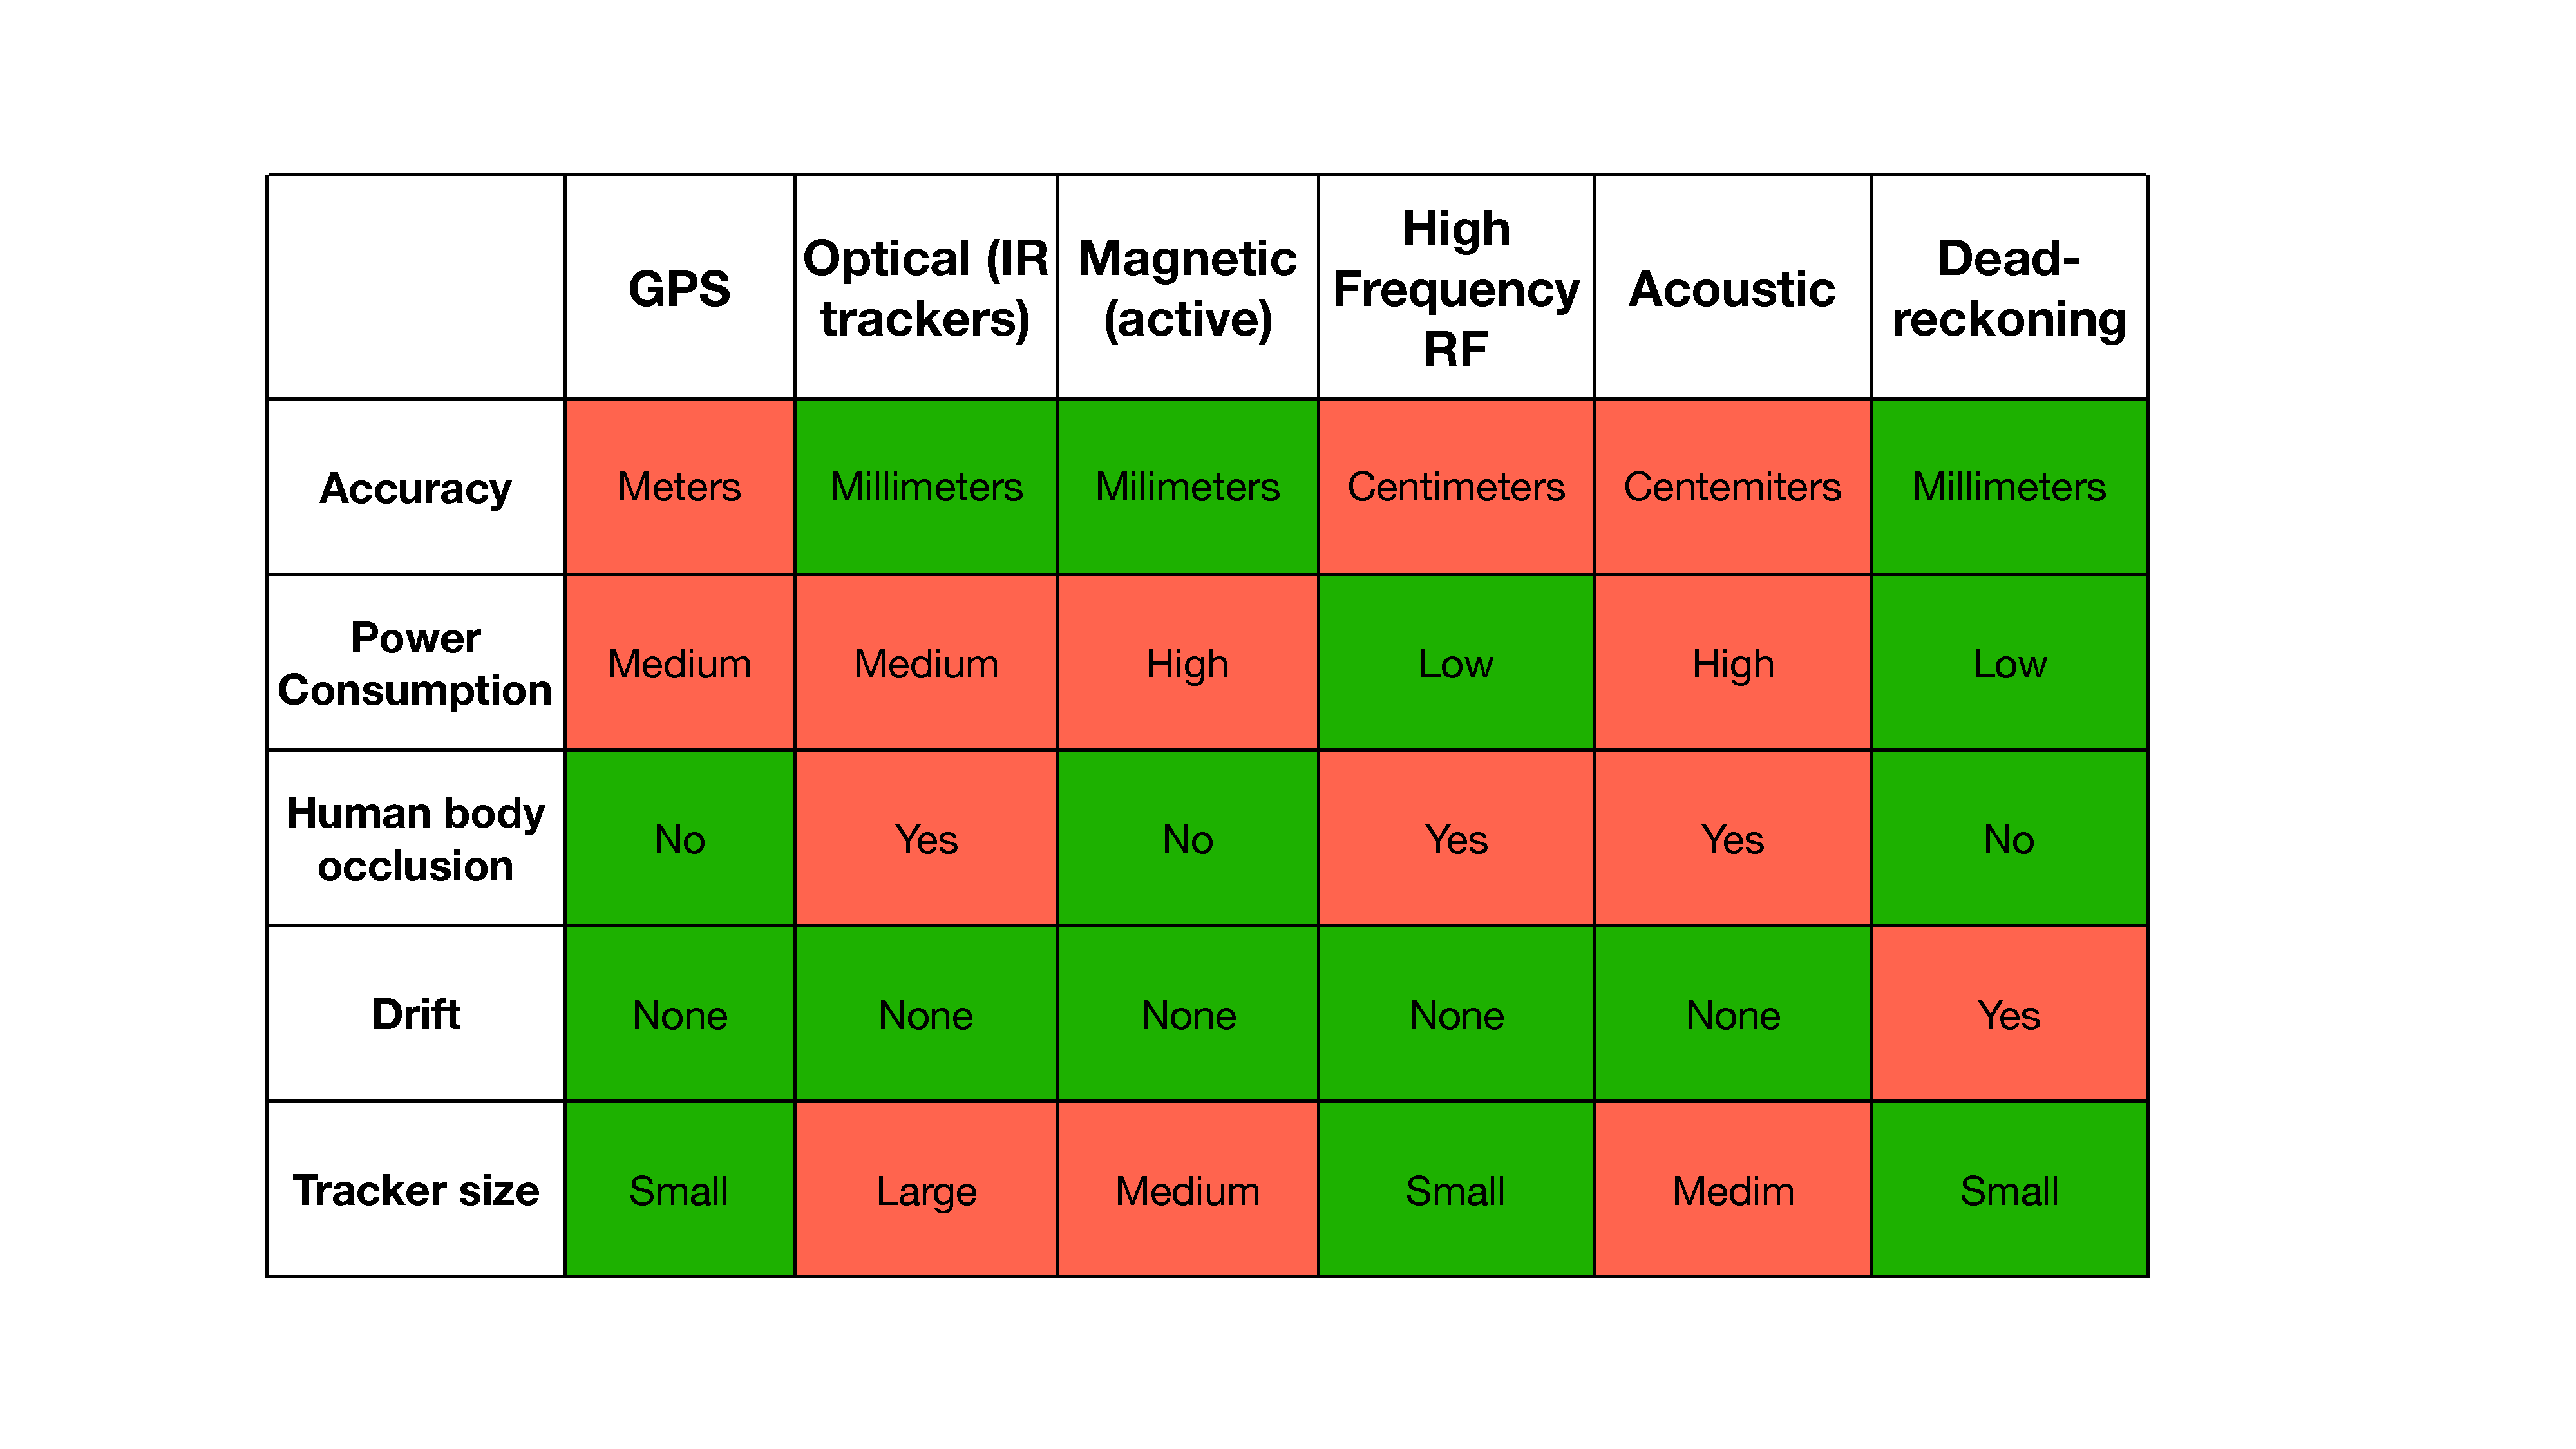
\includegraphics[width=14.0cm]{pictures/chapter5/pic_comparison_navigation.pdf}
\caption{Summary comparison of studied localization methods. The colors indicate if the specification satisfies DWT requirements. Green color is acceptable and red color is not. }
\label{fig:localization_compare}
\end{figure}

\section{Navigation design}
To attempt to satisfy our requirements, we designed a custom system. The system uses two methods: dead-reckoning for relative position and machine vision markers for providing absolute position. 

\begin{figure}[h]
\centering
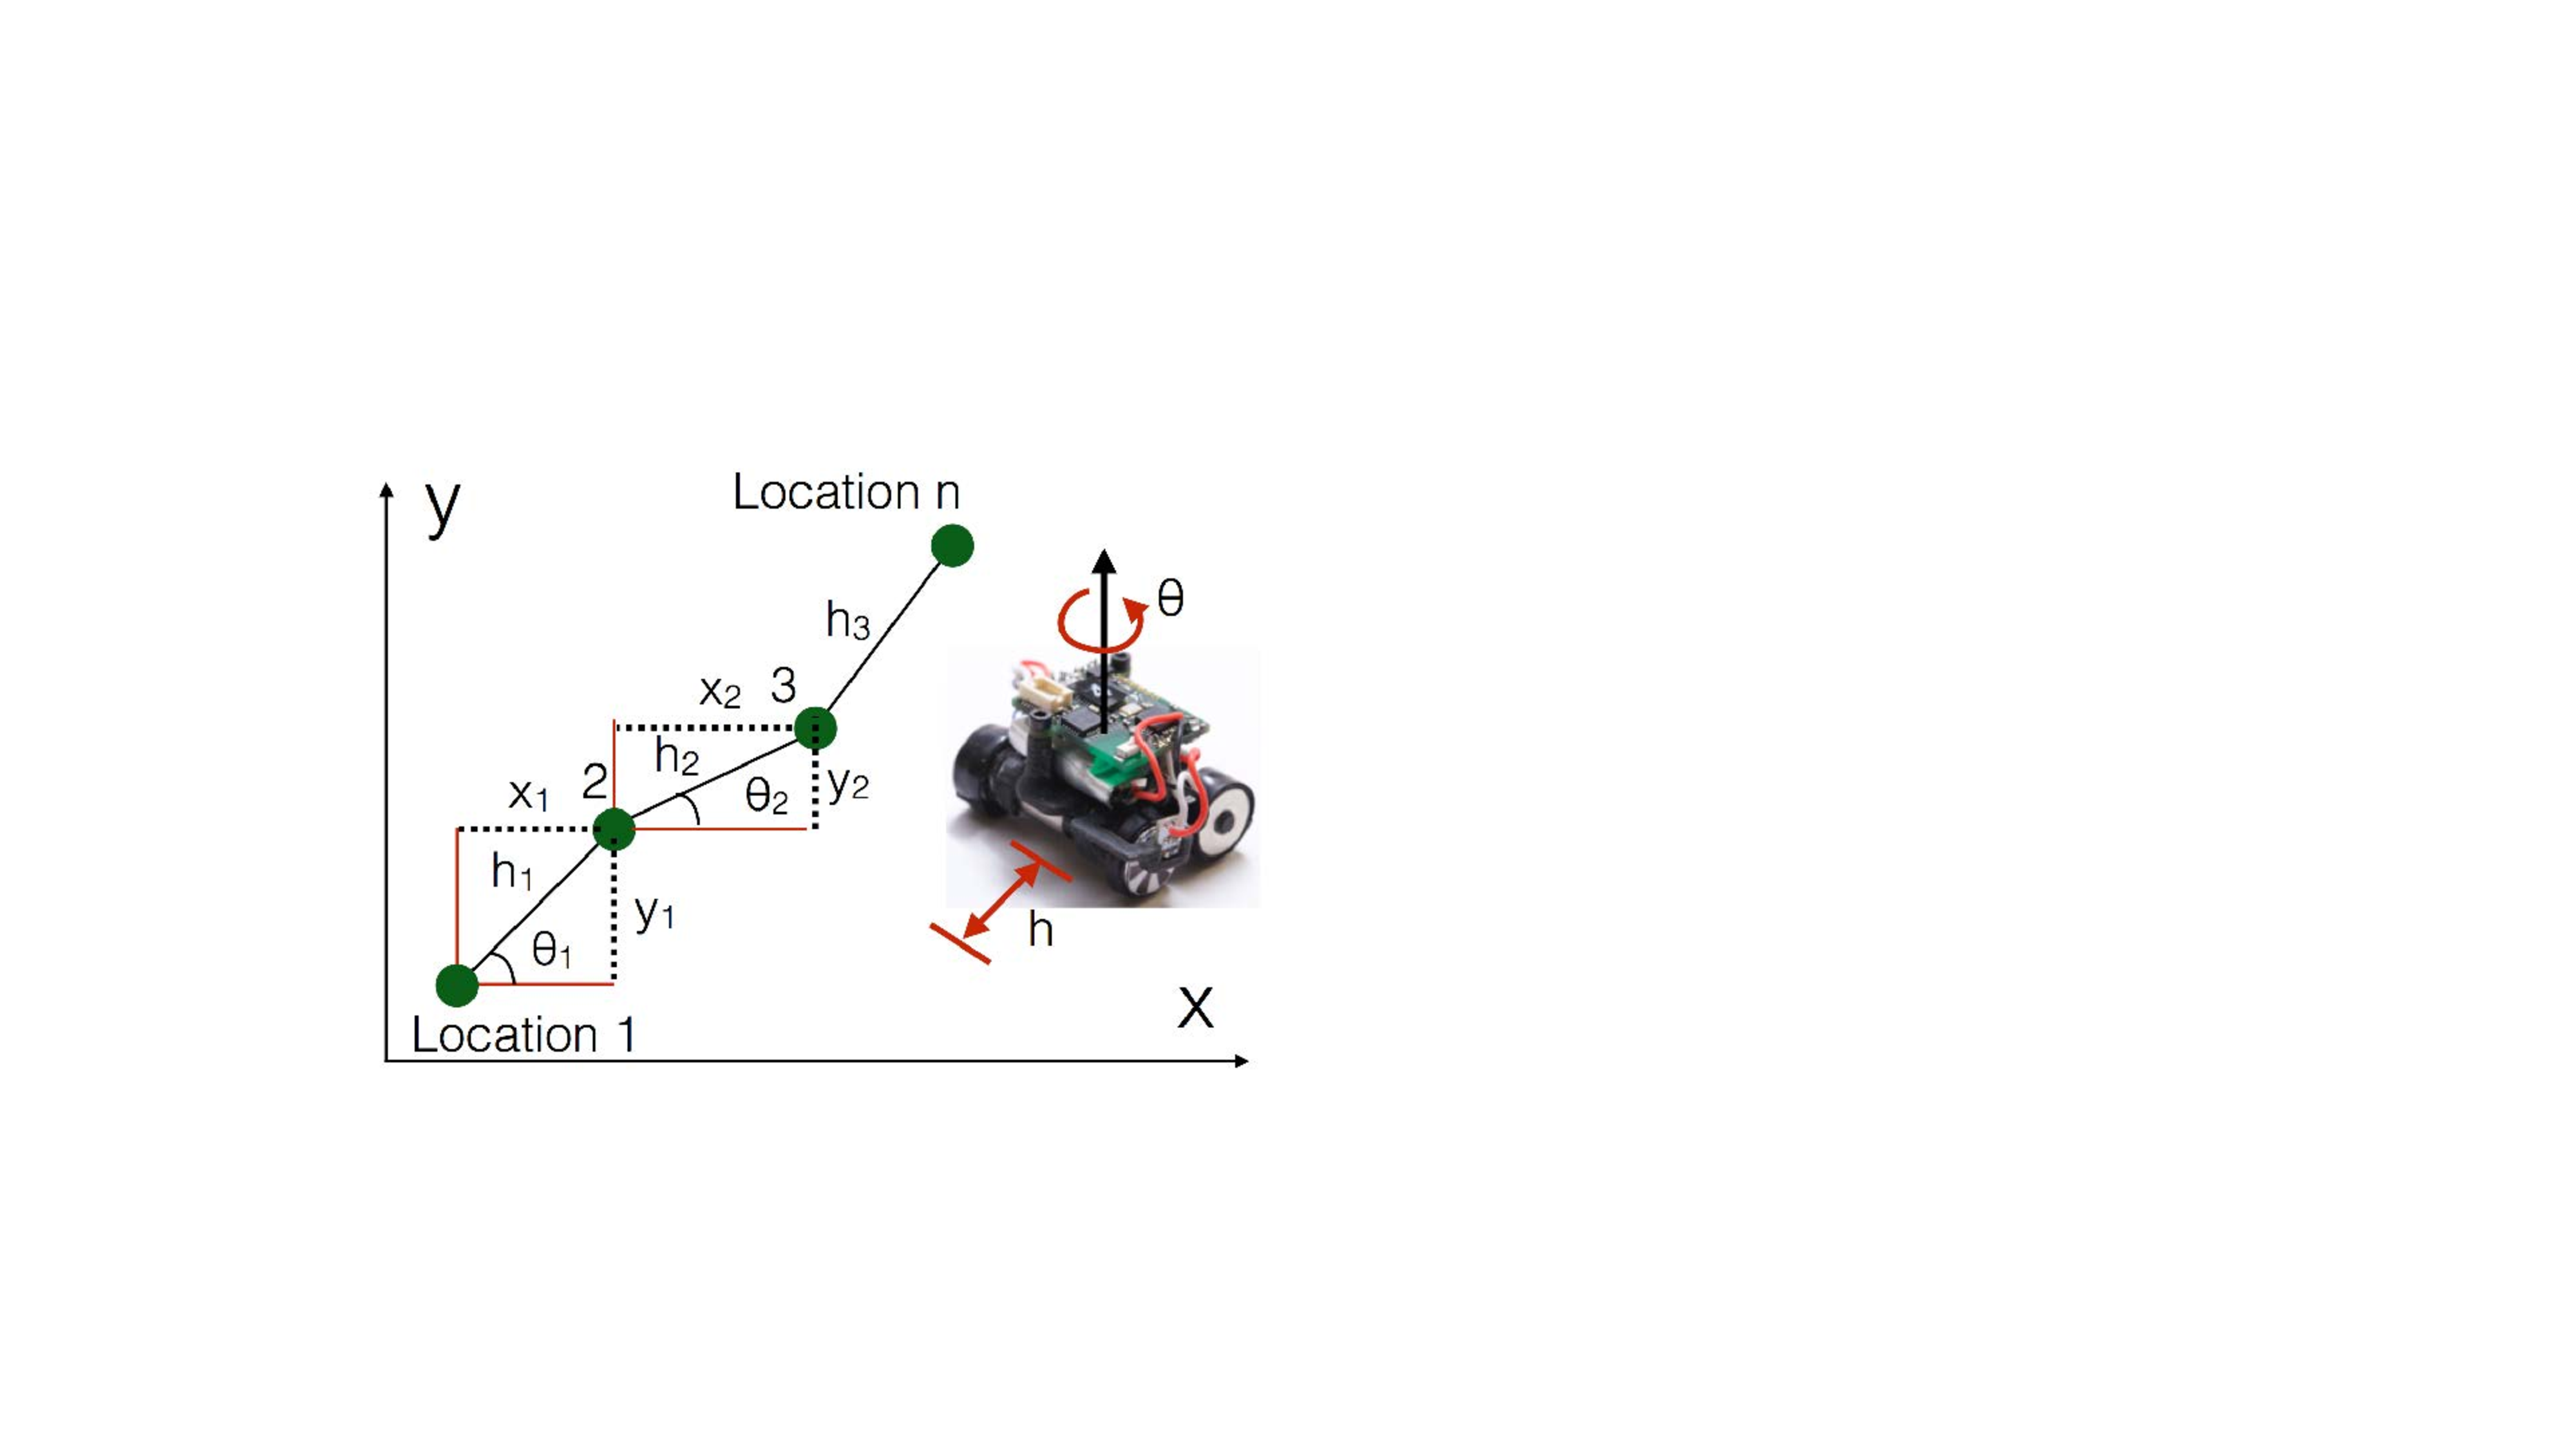
\includegraphics[width=8.0cm]{pictures/chapter5/visual_navigation.pdf}
\caption{The graphical representation of the dead-reckoning algorithm. The location is determined by previous location, yaw angle, and the traveled distance. }
\label{fig:graphical_dead_reck}
\end{figure}

\subsection{Dead-reckoning with inertial sensors and odometry}
In particular to DWT,  the dead-reckoning method estimates the position of the robot with the two following equations:
\[x_{n} = x_{n-1}+qh\cos(\theta_{n})\]
\[y_{n} = y_{n-1}+qh\sin(\theta_{n})\]
where $x$ and $y$ indicate the position in a 2D plane and $x_{n-1}$ and $y_{n-1}$ are the previous position estimates.  $h$ is the linear traveled distance, $\theta_n$ is the rotation angle, and $q$ is a scaling factor used for conversion of the sensor data onto centimeters. Figure~\ref{fig:graphical_dead_reck} shows how this algorithm works in practice for three consequative approximations. 

 The linear distance is obtained from the encoders on the motors. The rotation angle is obtained by integrating the gyroscope x-axis rotation rate and using the following equation: 
\[\theta_{n}=\theta_{n-1}+d\theta_{n}-ct\]
where $c$ is the gyroscope drift constant, which we measured by logging stationary gyroscope rotation angle, $t$ is the elapsed time, and $d\theta_{n}$ is the gyro rotation rate. Specifically, we used a 3-axis accelerometer and 3-axis gyroscope (MPU6050, Invensense). We did not include a magnetometer, because of possible interference nearby magnetic wheels.   Since dead-reckoning is based on integration, any errors will accumulate over time. 

Although, in reality, the robot moves in 3D, the 2D navigation is easier to employ in practice and use for estimation. We assume that the robot is always bound to some surface. With small step approximation, the surface can be unwrapped in 2D, whether the fabric or human body  

\subsection{Getting a map}
As with most navigation, the map of the space is required to make sense of the position estimates. For the clothing robots obtaining the map is straightforward. Almost all clothing is made from 2D sheets of fabric that are sewn together. The original templates that were used to make the clothing can be used as a map. 
Getting a map of the body is harder, as every individual is different. The body map can be obtained from a 3D scanner. In particular, we used an affordable off-the-shelf scanner (Sense 3D, 3D Systems). With this scanner, we could digitalize a hand or head. For a whole body, a stationary scanner is needed, as the human subject cannot remain completely still during scanning. There are few such booths for commercial use (Shapify Booth, Artec 3D)   Alternatively, a body map can be obtained using photogrammetry~\cite{mikhail2001introduction}, where photos from different angles are stitched together into a 3D mesh. 

The map is represented as a triangulated surface mesh, as it is obtained from a 3D scanner or a generated model. Such representation is the easiest to manipulate programmatically and provides the best approximation of the complex geometry of the human body. Each vertex has x,y,z coordinates as well as information on connections with neighboring triangles. 

After the map is obtained, localization of SkinBot is as follows: 1)~the robot's coordinates are scaled to the texture map, 2)~all the texture coordinates were searched to find X-Y coordinates in the vicinity of robot's coordinates. 3)~the Euclidean distance\footnote{$d(x,y)=\sqrt[]{(x_1-x_2)^2+(y_1-y_2)^2}$} between the found X-Y neighboring coordinates and robot coordinates were computed, and 4)~the coordinate with the smallest Euclidean distance to the robot was assumed to be the robot's location. Therefore the robot moves by jumping from different vertices, and the density of the vertices limits the resolution. 

\begin{figure}[!ht]
\centering
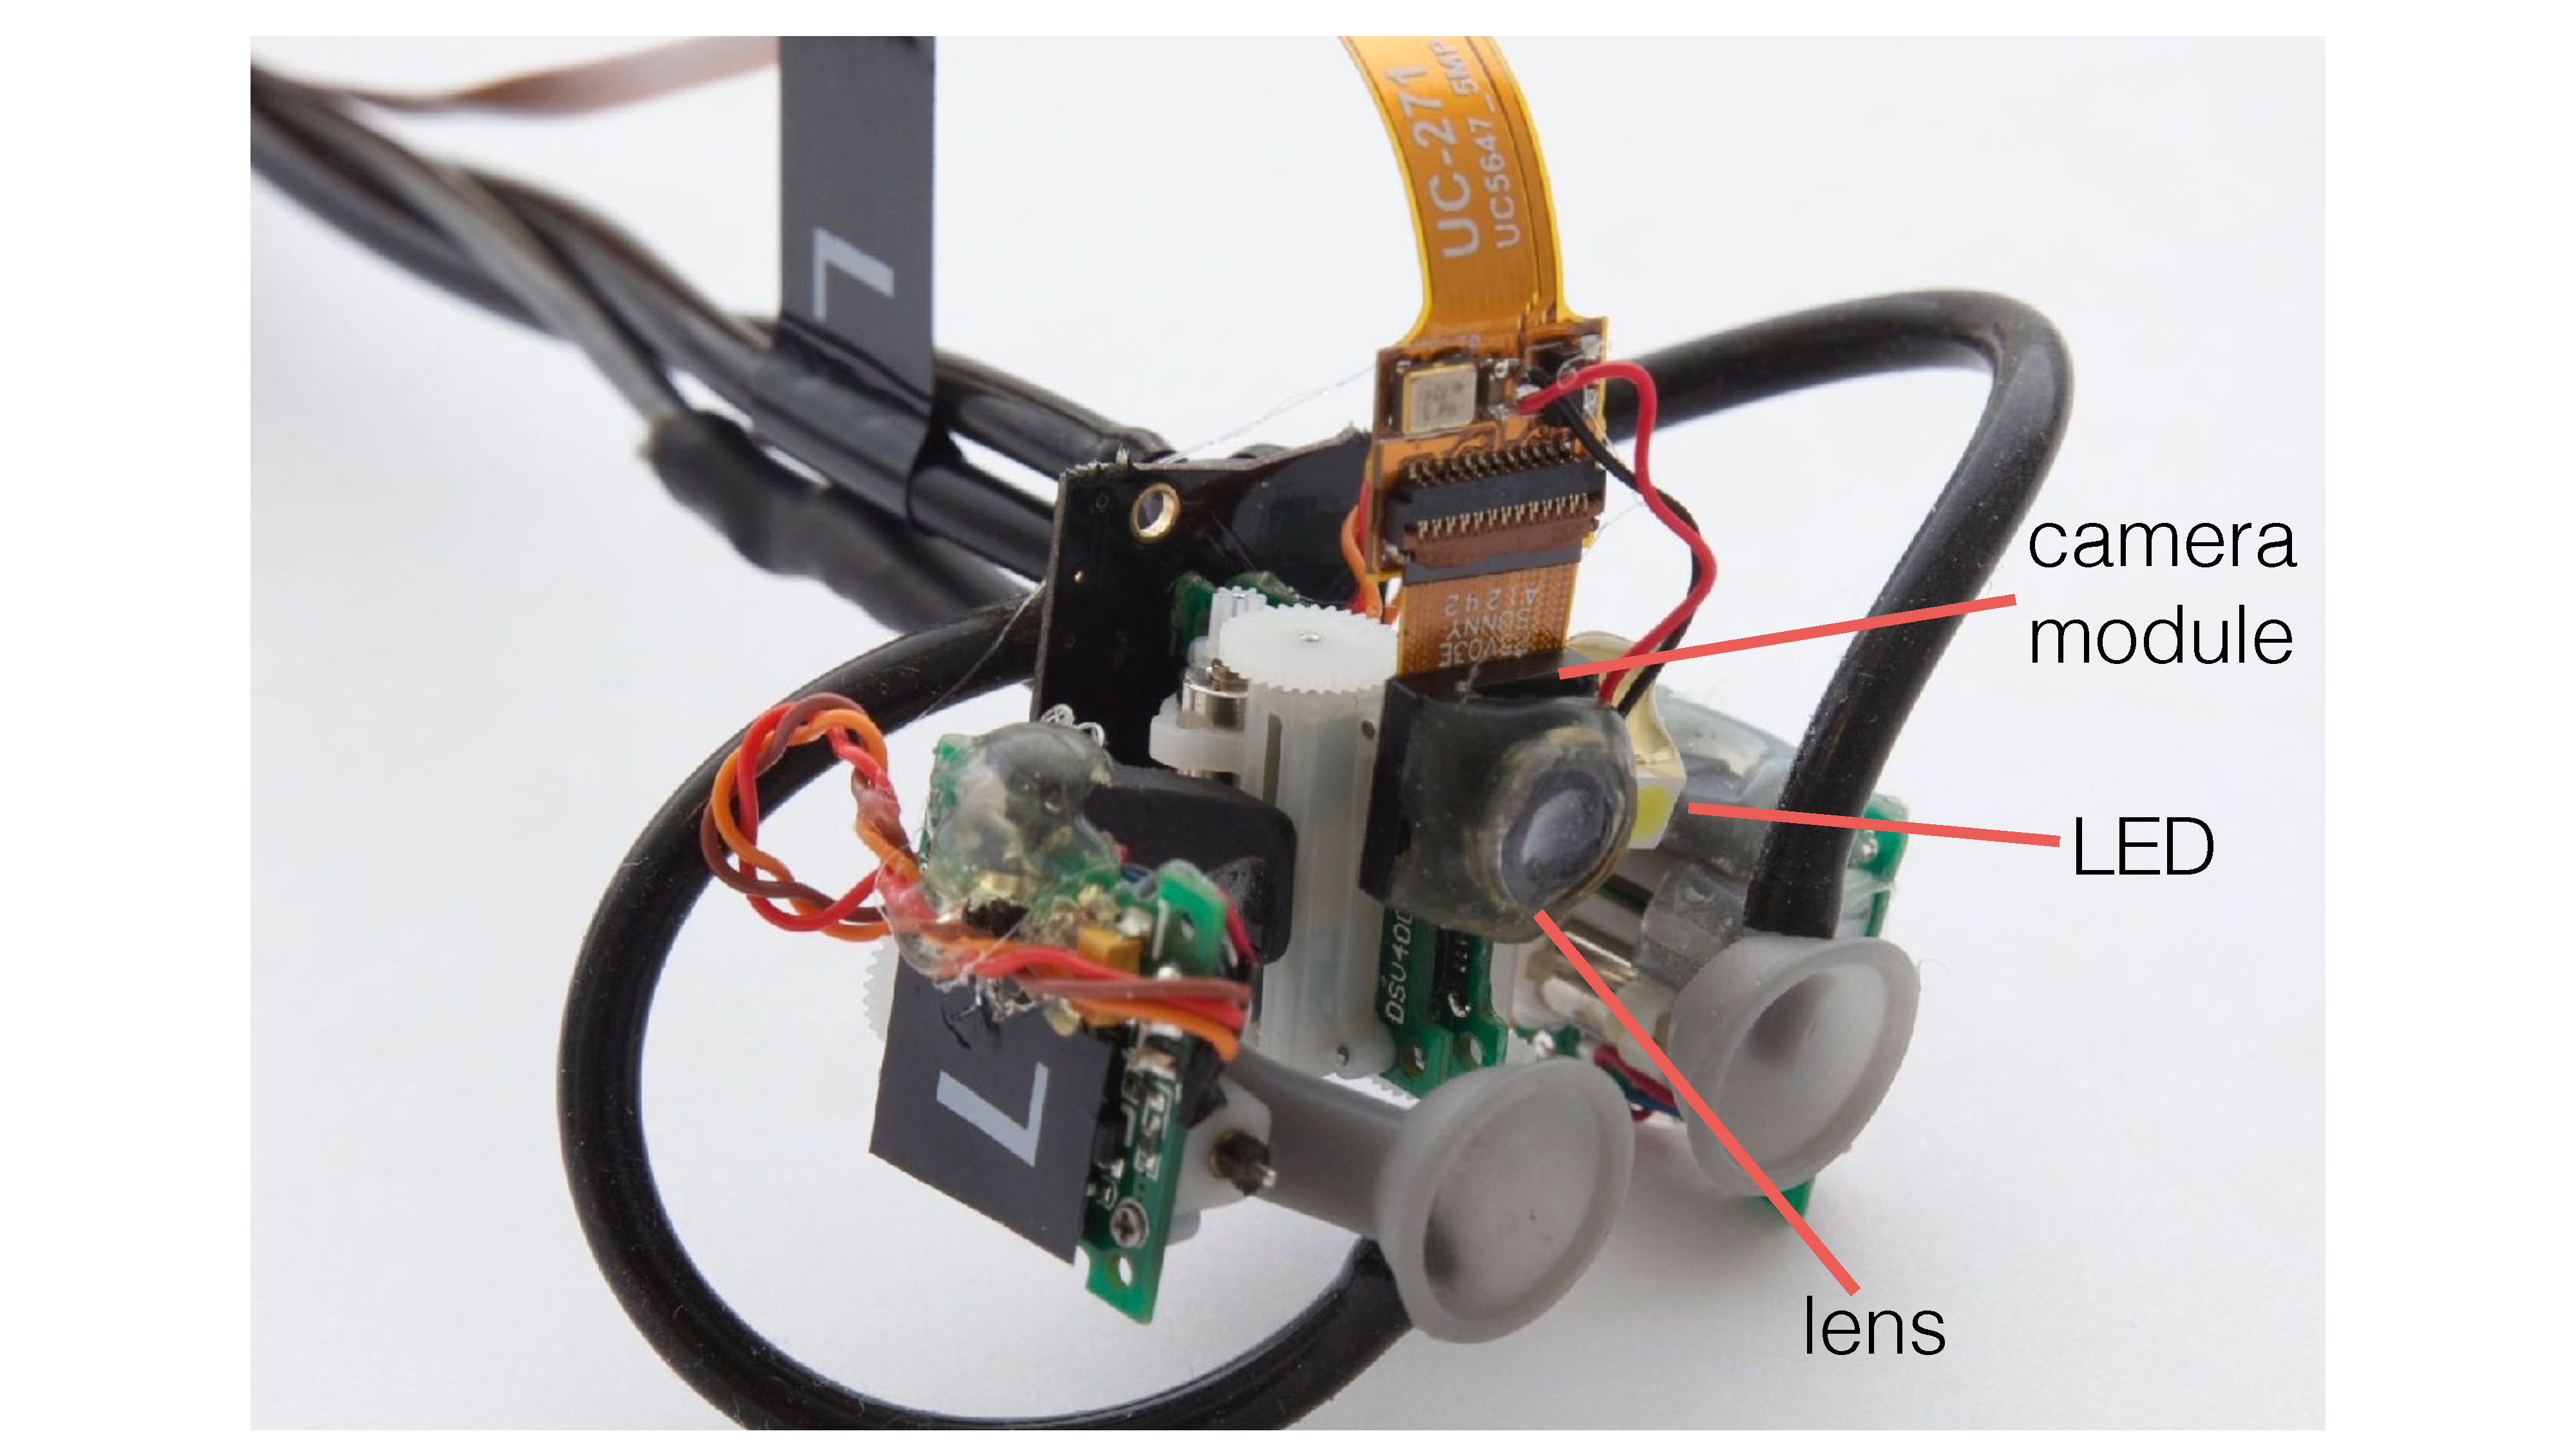
\includegraphics[width=10.0cm]{pictures/chapter5/camera_pic.pdf}
\caption{Picture of the robot equiped with the camera }
\label{fig:pic_camera}
\end{figure}

\subsection{Passive navigation markers}
Dead-reckoning provides only relative position and will accumulate drift. To alleviate these issues, some absolute position sensing is required. We employ a method of placing markers on the fabric or the body in the predetermined locations. The markers reset the robot's dead-reckoning errors as well as provide an anchor to the digital map. Each marker contains heading and distance information. 

In particular, we printed markers on temporary tattoo paper (A4 Laser Printer, RoryTory) which does not interfere with the robot's suction of the skin and are easily removed. The markers are 2cm in diameter. We designed a visible guide for initial manual robot placement and fiducials to recalibrate the robot's dead-reckoning position, as shown in Fig.~\ref{fig:fidual_markers}~. The fiducials are recognized with the robot's camera, as shown in Figure~\ref{fig:pic_camera} and custom machine vision methods (OpenCV 3.4.1) that run on Raspberry PI 3. 

\begin{figure}[!ht]
\centering
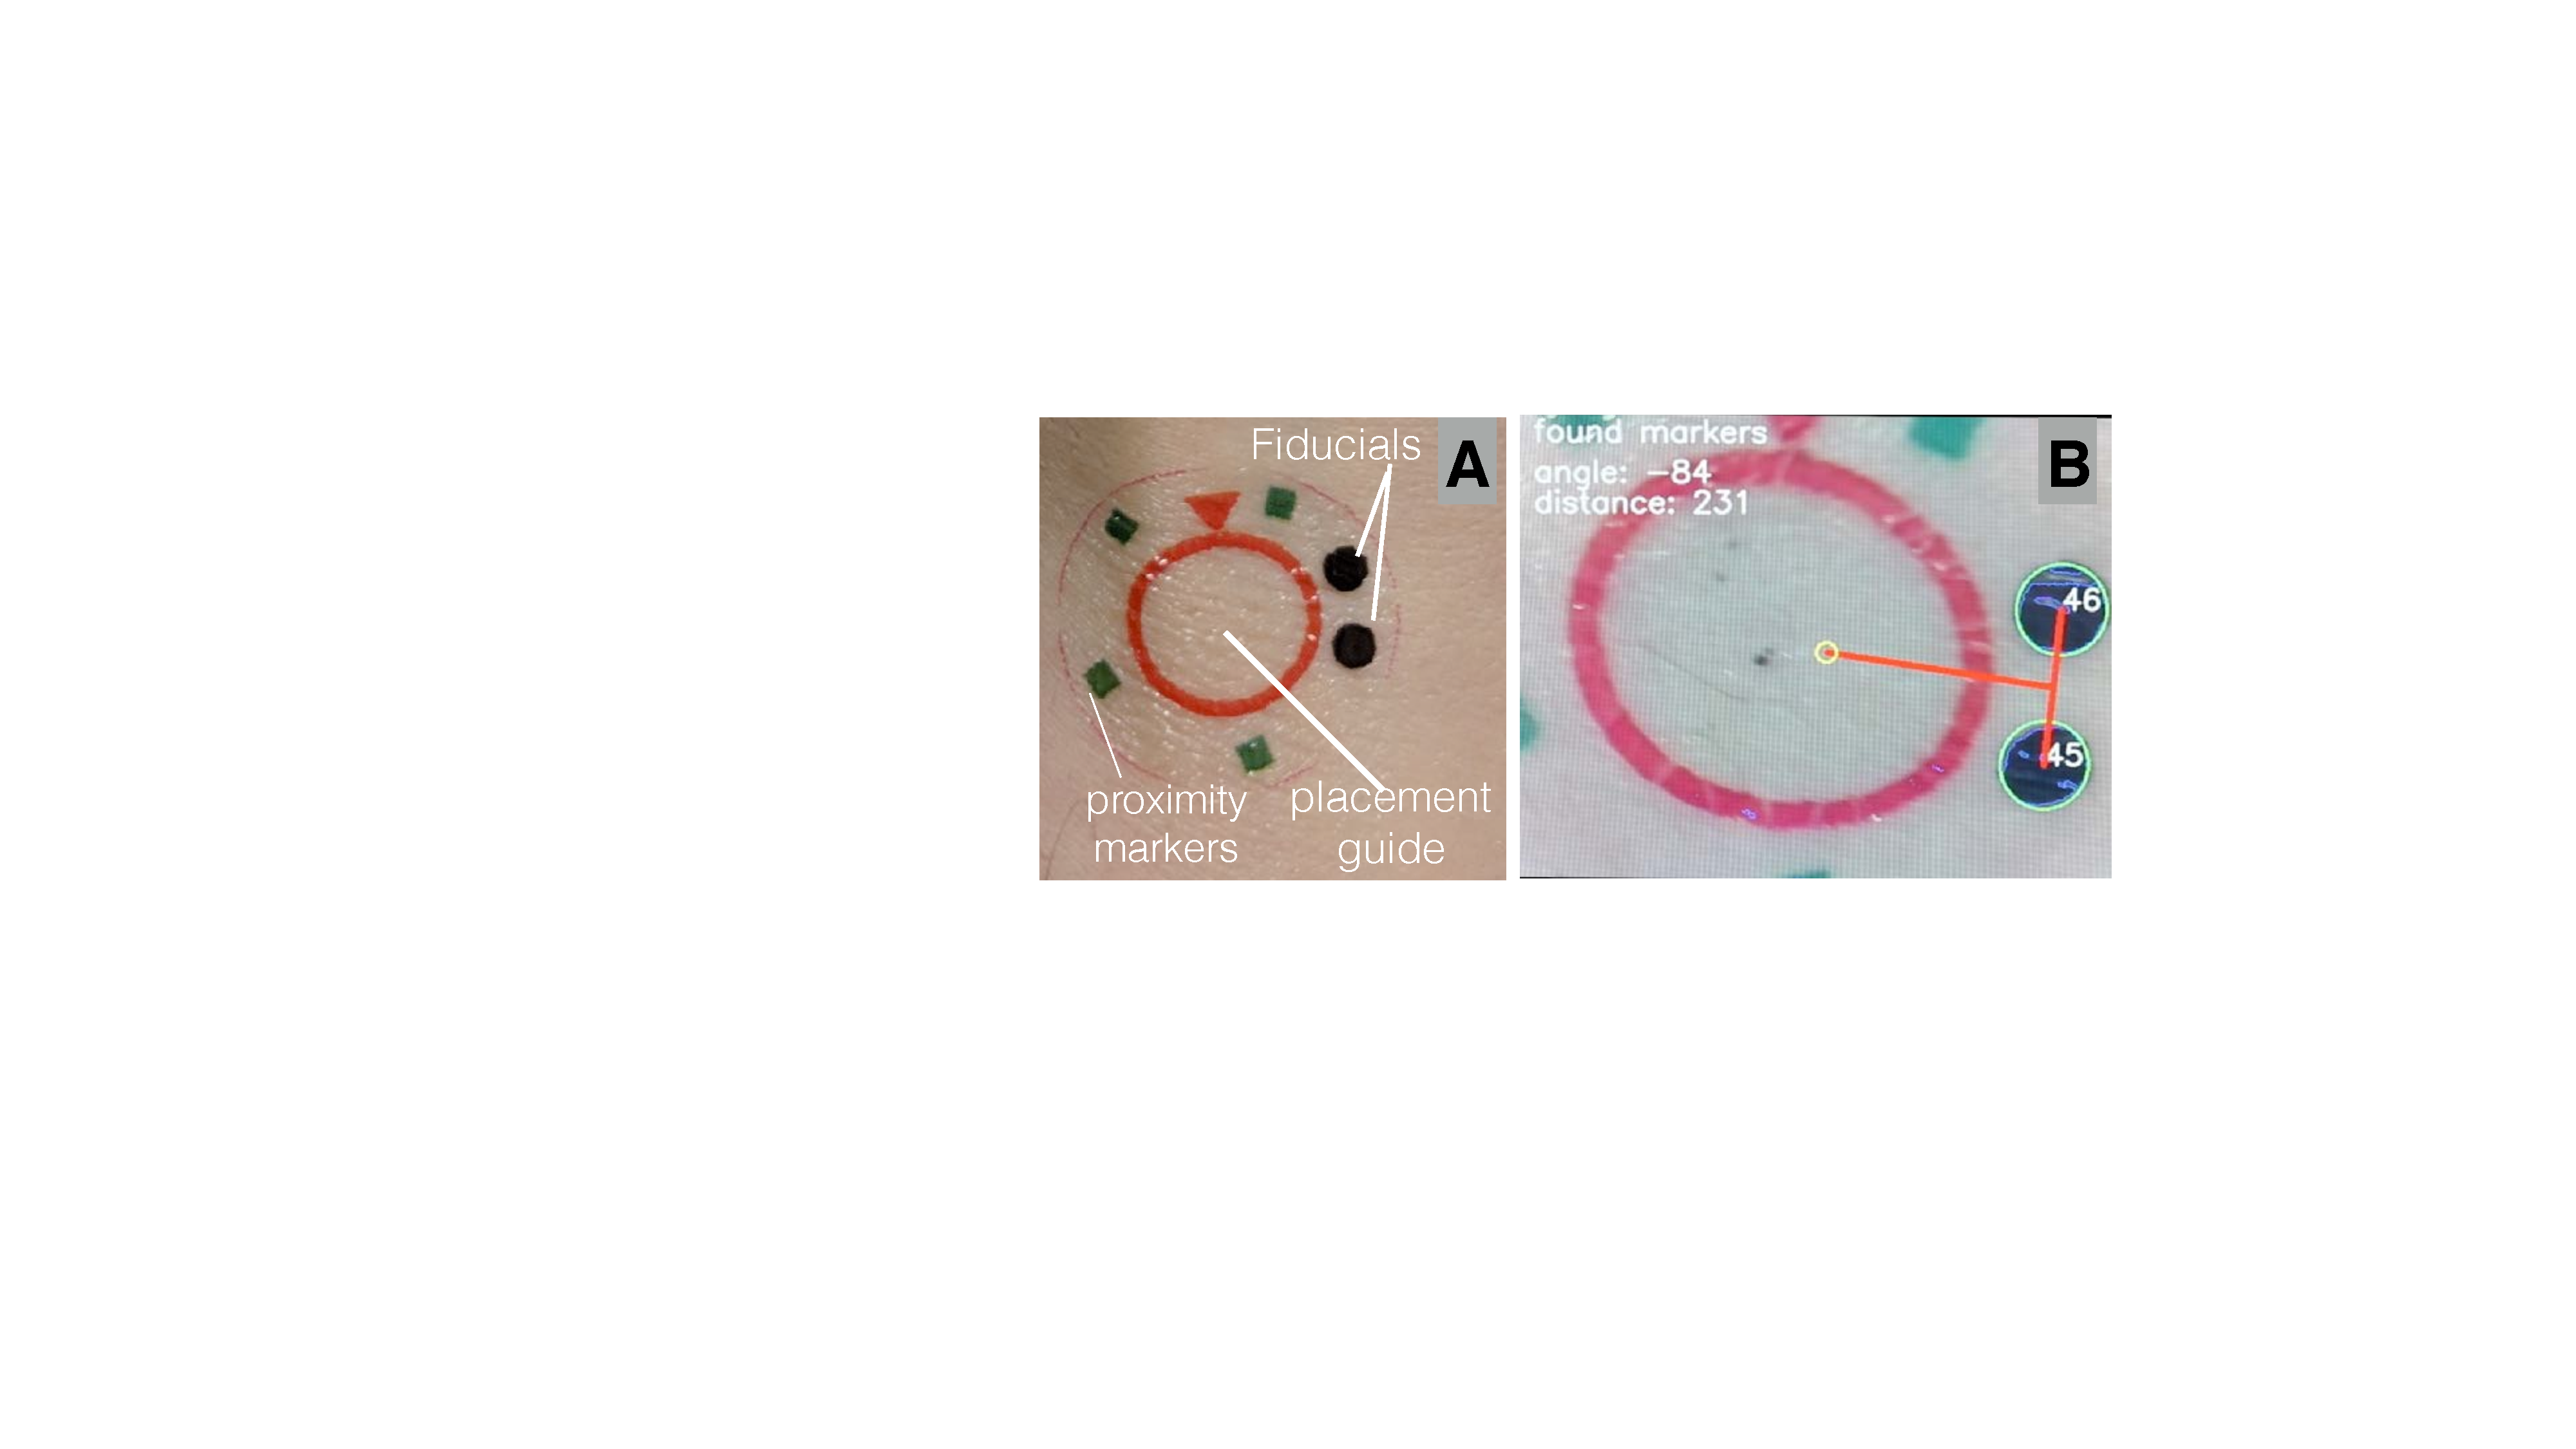
\includegraphics[width=11.0cm]{pictures/chapter5/fidutial_markers.pdf}
\caption{Temporary tattoo markers. a)Closeup of the marker. The fiduals and proximity markers are for the camera. The red placement guide is for initial robot placement. b) The marker as seen by the machine vision. }
\label{fig:fidual_markers}
\end{figure}


The markers were used in the following steps:  
1) The camera image was grayscaled and thresholded to look for black color only 
2) The contours on the thresholded image were computed. 
3) If contour was a circle of a predefined size, it meant it was the fiducial. 
4) The centers of the two fiducials were calculated
5) A line was drawn between the two fiducial centers. To that line, a perpendicular line was drawn to the center of the view. 
6) The length of the perpendicular line was used as the robot distance offset. 
7) The angle of the perpendicular line was used as the angle offset. 

Due to the drift of the dead-reckoning, it might be hard to find the position of the fiducials. The green proximity markers helped to find the fiducial markers, as they indicated that the fiducials markers are nearby, even if they are not in view. 

To anchor to the 3D map the markers have to be placed in the predefined position and rotation. Currently, such markers would have to be placed manually, as shown in the Figure~\ref{fig:guide_markers}. To visually guide consistent placement, we printed black-colored guides on the cover of the temporary tattoo marker.  We developed a simple smartphone (Google Pixel 2 with Android 8.1.0) camera application which shows a contour of the hand and where to place the marker. The user aligns their hand with the contour on the camera for the marker placement.
The contour guide is automatically generated from the 3D map.
With the clothing, it is simpler to position the markers. The markers can be placed permanently during the manufacturing of the clothing. With digital manufacturing such as flat-bed knitting machines, the markers can be stitched into clothing directly. 





\begin{figure}[!ht]
\centering
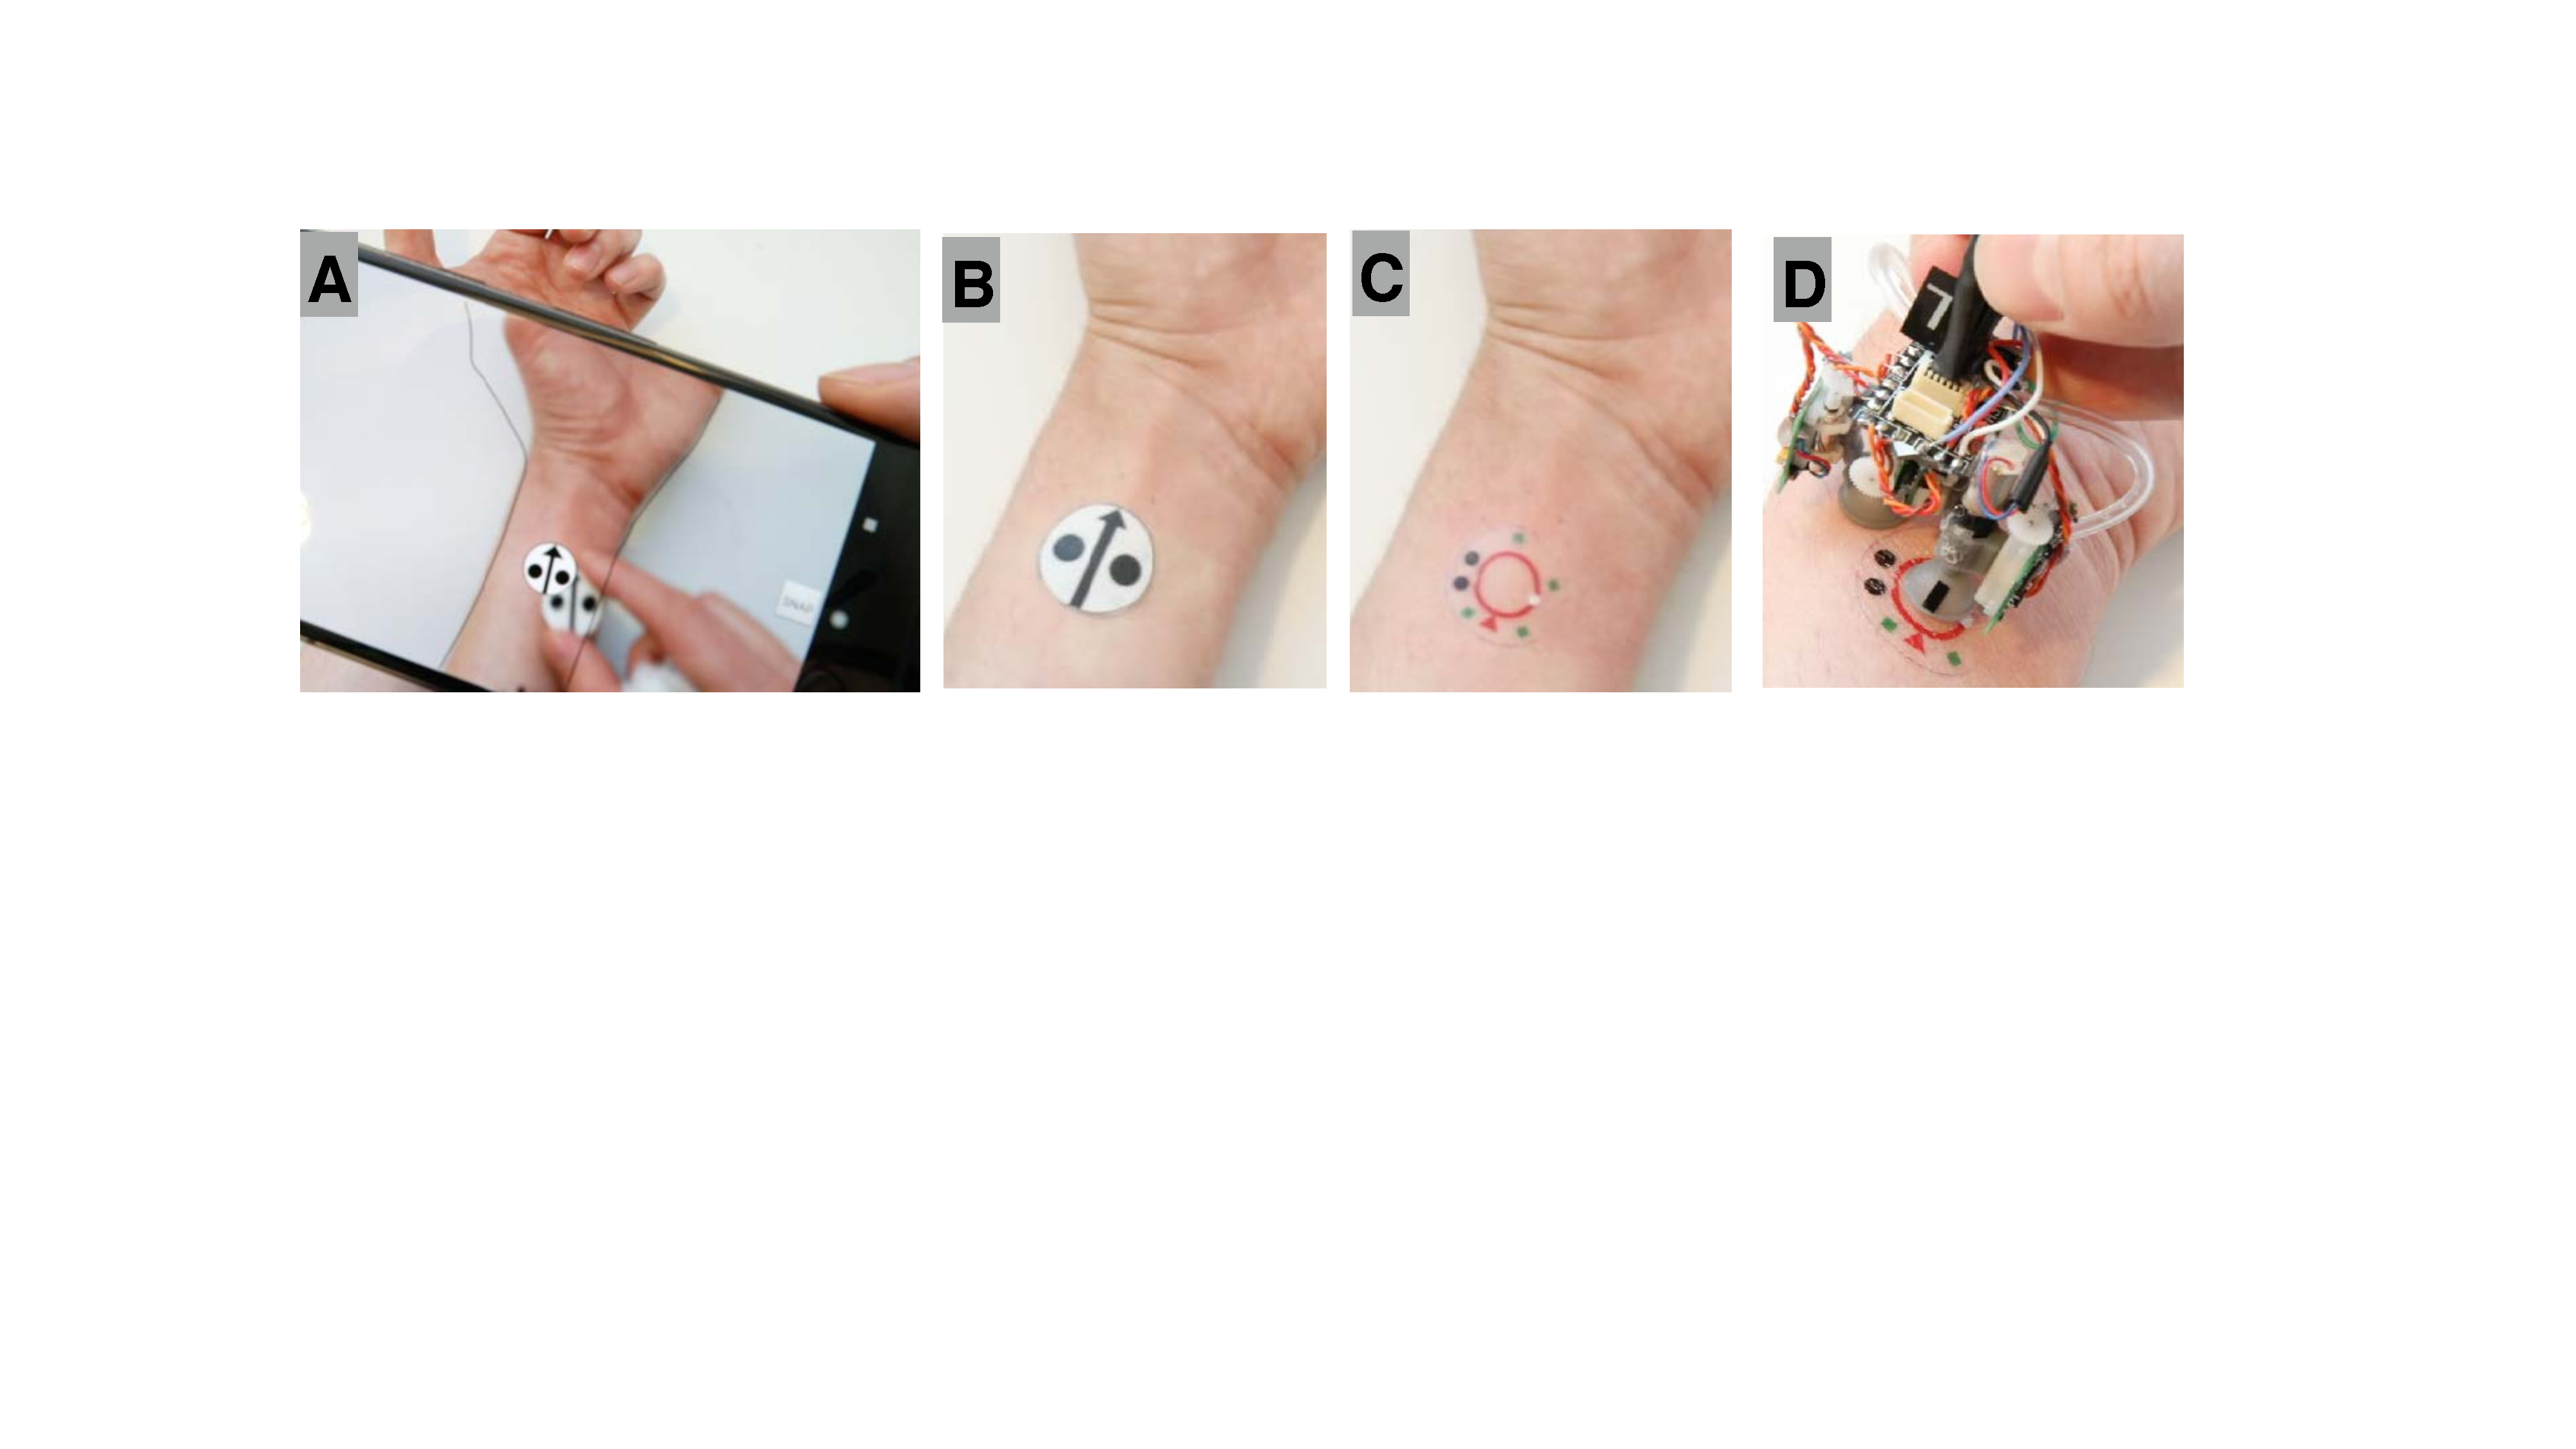
\includegraphics[width=14.0cm]{pictures/chapter5/marker_placement.pdf}
\caption{Guided attachment of the markers. a) The phone is used to guide the placement. The cover of the marker has a sticker for visual rotation. b) The marker is attached before the sticker is removed c) The cover sticker is removed d) The robot is placed on the marker as the starting point.  }
\label{fig:guide_markers}
\end{figure}



\subsection{Active navigation markers}
Initially, we have considered and designed active navigation markers as well. The main advantage of active markers is that it can signal its position to the robot remotely, so the robot does not need to be close to the marker to use it. The main disadvantage is higher power consumption, as well as an additional piece of hardware. Furthermore, it would be hard to attach to the skin, unless it is in the form of bracelet or another wearable. 

\begin{figure}[!ht]
\centering
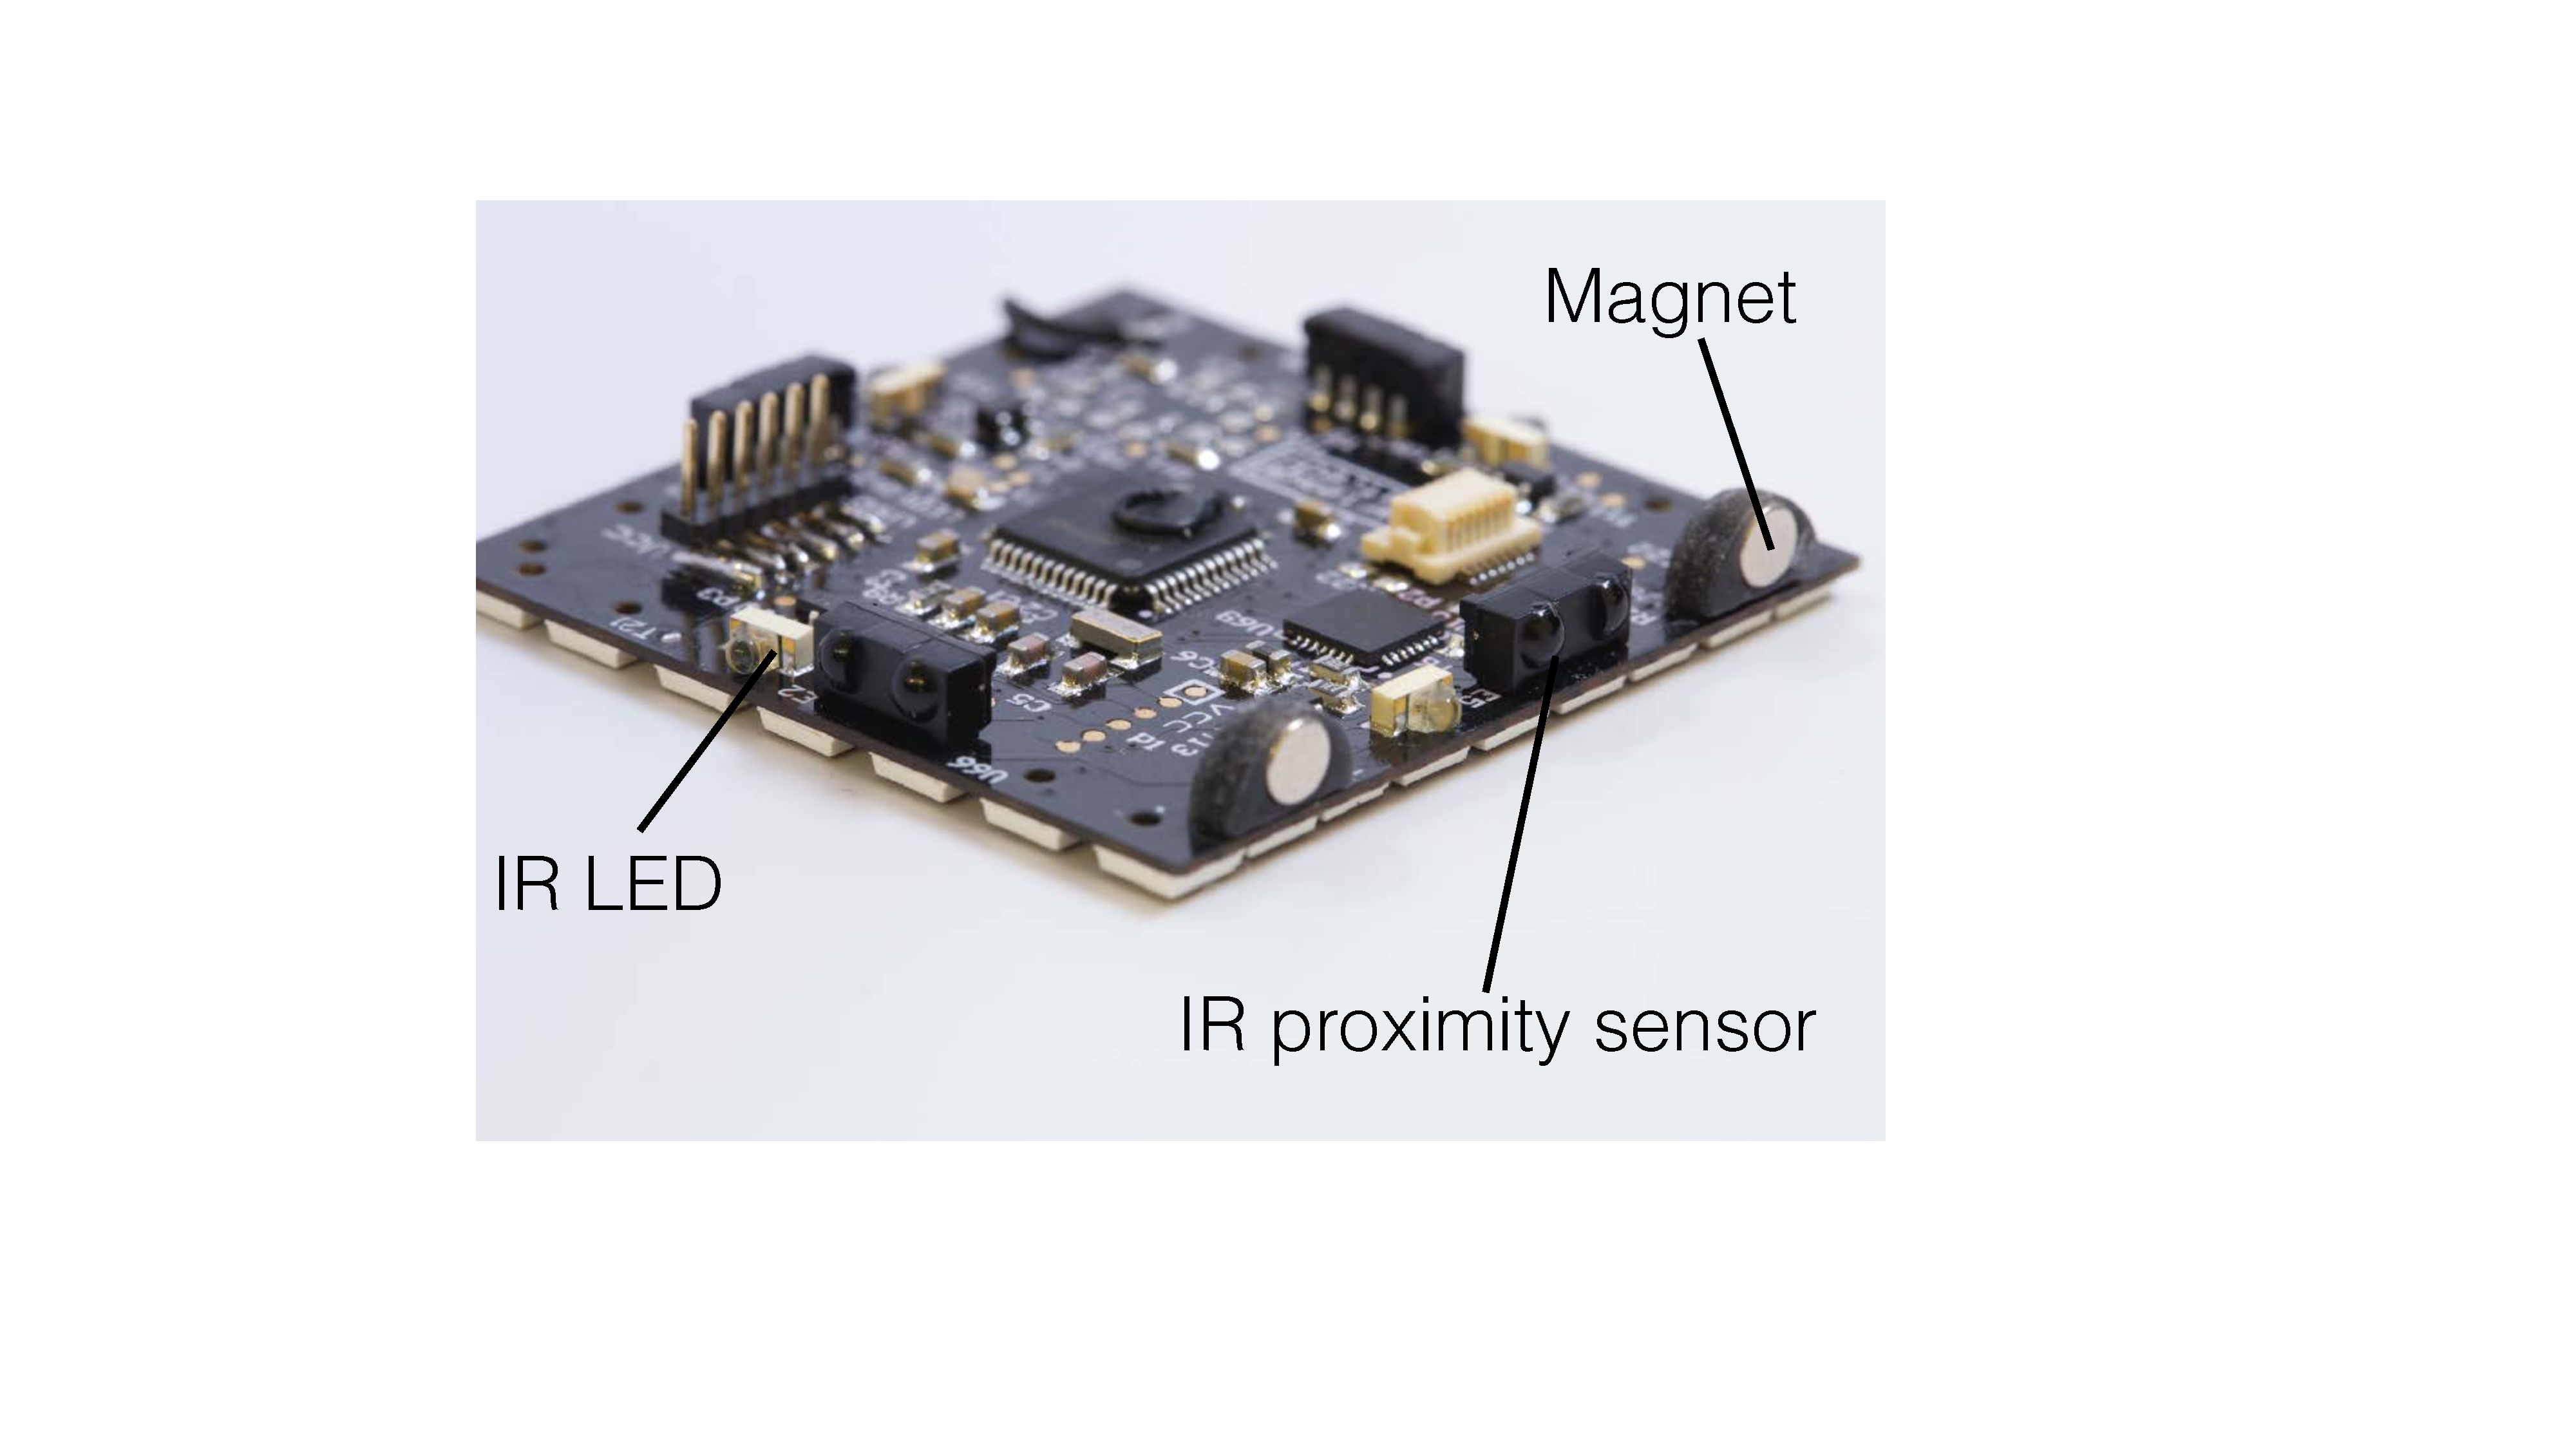
\includegraphics[width=9.0cm]{pictures/chapter5/ir_beacons.pdf}
\caption{Four infrared proximity sensors for active navigation markers.}
\label{fig:active_beacons}
\end{figure}

We used infrared (IR) active markers as shown in Figure~\ref{fig:active_beacons}. The Rovables robot was equipped with 4 IR proximity sensors (TSSP77P38, Vishay) on each side. This sensor measured the intensity of 38kHz modulated infrared light at 940nm. A 940nm  directional infrared LED light source was pinned to the clothing to work as the navigation marker. By measuring the intensity of the light on each side, the robot can determine the direction of the light, as well as the distance from the intensity. 

In practice, intensity-based infrared proximity is unreliable~\footnote{As seen in the kitchen taps and toilet flush}. A more sophisticated time-of-flight approach would be more appropriate. Most fabrics are very reflective in the infrared spectrum. It is challenging to determine the location of the beacon, as there are many reflective paths the IR light takes. 

\subsection{Localization during body motion}
The motion of the body will throw off the gyroscope measurements; therefore, the current dead-reckoning can only be performed on the stationary body. If any external motion is detected, the robot stops and turns off the gyroscope integration. When no motion is detected, the robot resumes its course. 

The external motion is classified with the IMU. During localization, the accelerometer is sampled for sudden changed by thresholding the derivative of acceleration. 

\subsection{Path planning}
The computer (server) does not control the movement of the robots directly. It transmits the commands for the robots to accomplish. This is because the radio communication can be faulty and unpredictable as well as latency. The server also keeps tracks of the overall map and where robots are in relation to each other.

In the current implementation, path-planning is simple. The robot takes the shortest path to the destination. There are three basic commands: (1) move specified distance forward,  (2) move specified distance backward, and (3) turn to a specific angle. Using these three movements, a complex path can be followed. Each of the three movements was executed with different PID (proportional-integral-derivative) controllers. Without the PID controller, the robot would not follow a straight path, as the fabric surface is not even, and motors are not symmetrical. The IMU yaw angle was used to correct the course. Also, the yaw angle was used to control turning.  



\subsection{Localization with external optical system}
Since with localization, there are always tradeoffs. In some cases, it is acceptable to have external trackers. Some reasons might include: Person is confined to one room or cannot move. Submillimeter accuracy or high update rate($>$100Hz) is required. 3) Development and system validation. 

We used an optical motion capture system (Optitrack). We equipped the robots with 4 reflective markers as seen in Figure~\ref{fig:skinbot_reflective_markers}. 

\begin{figure}[!ht]
\centering
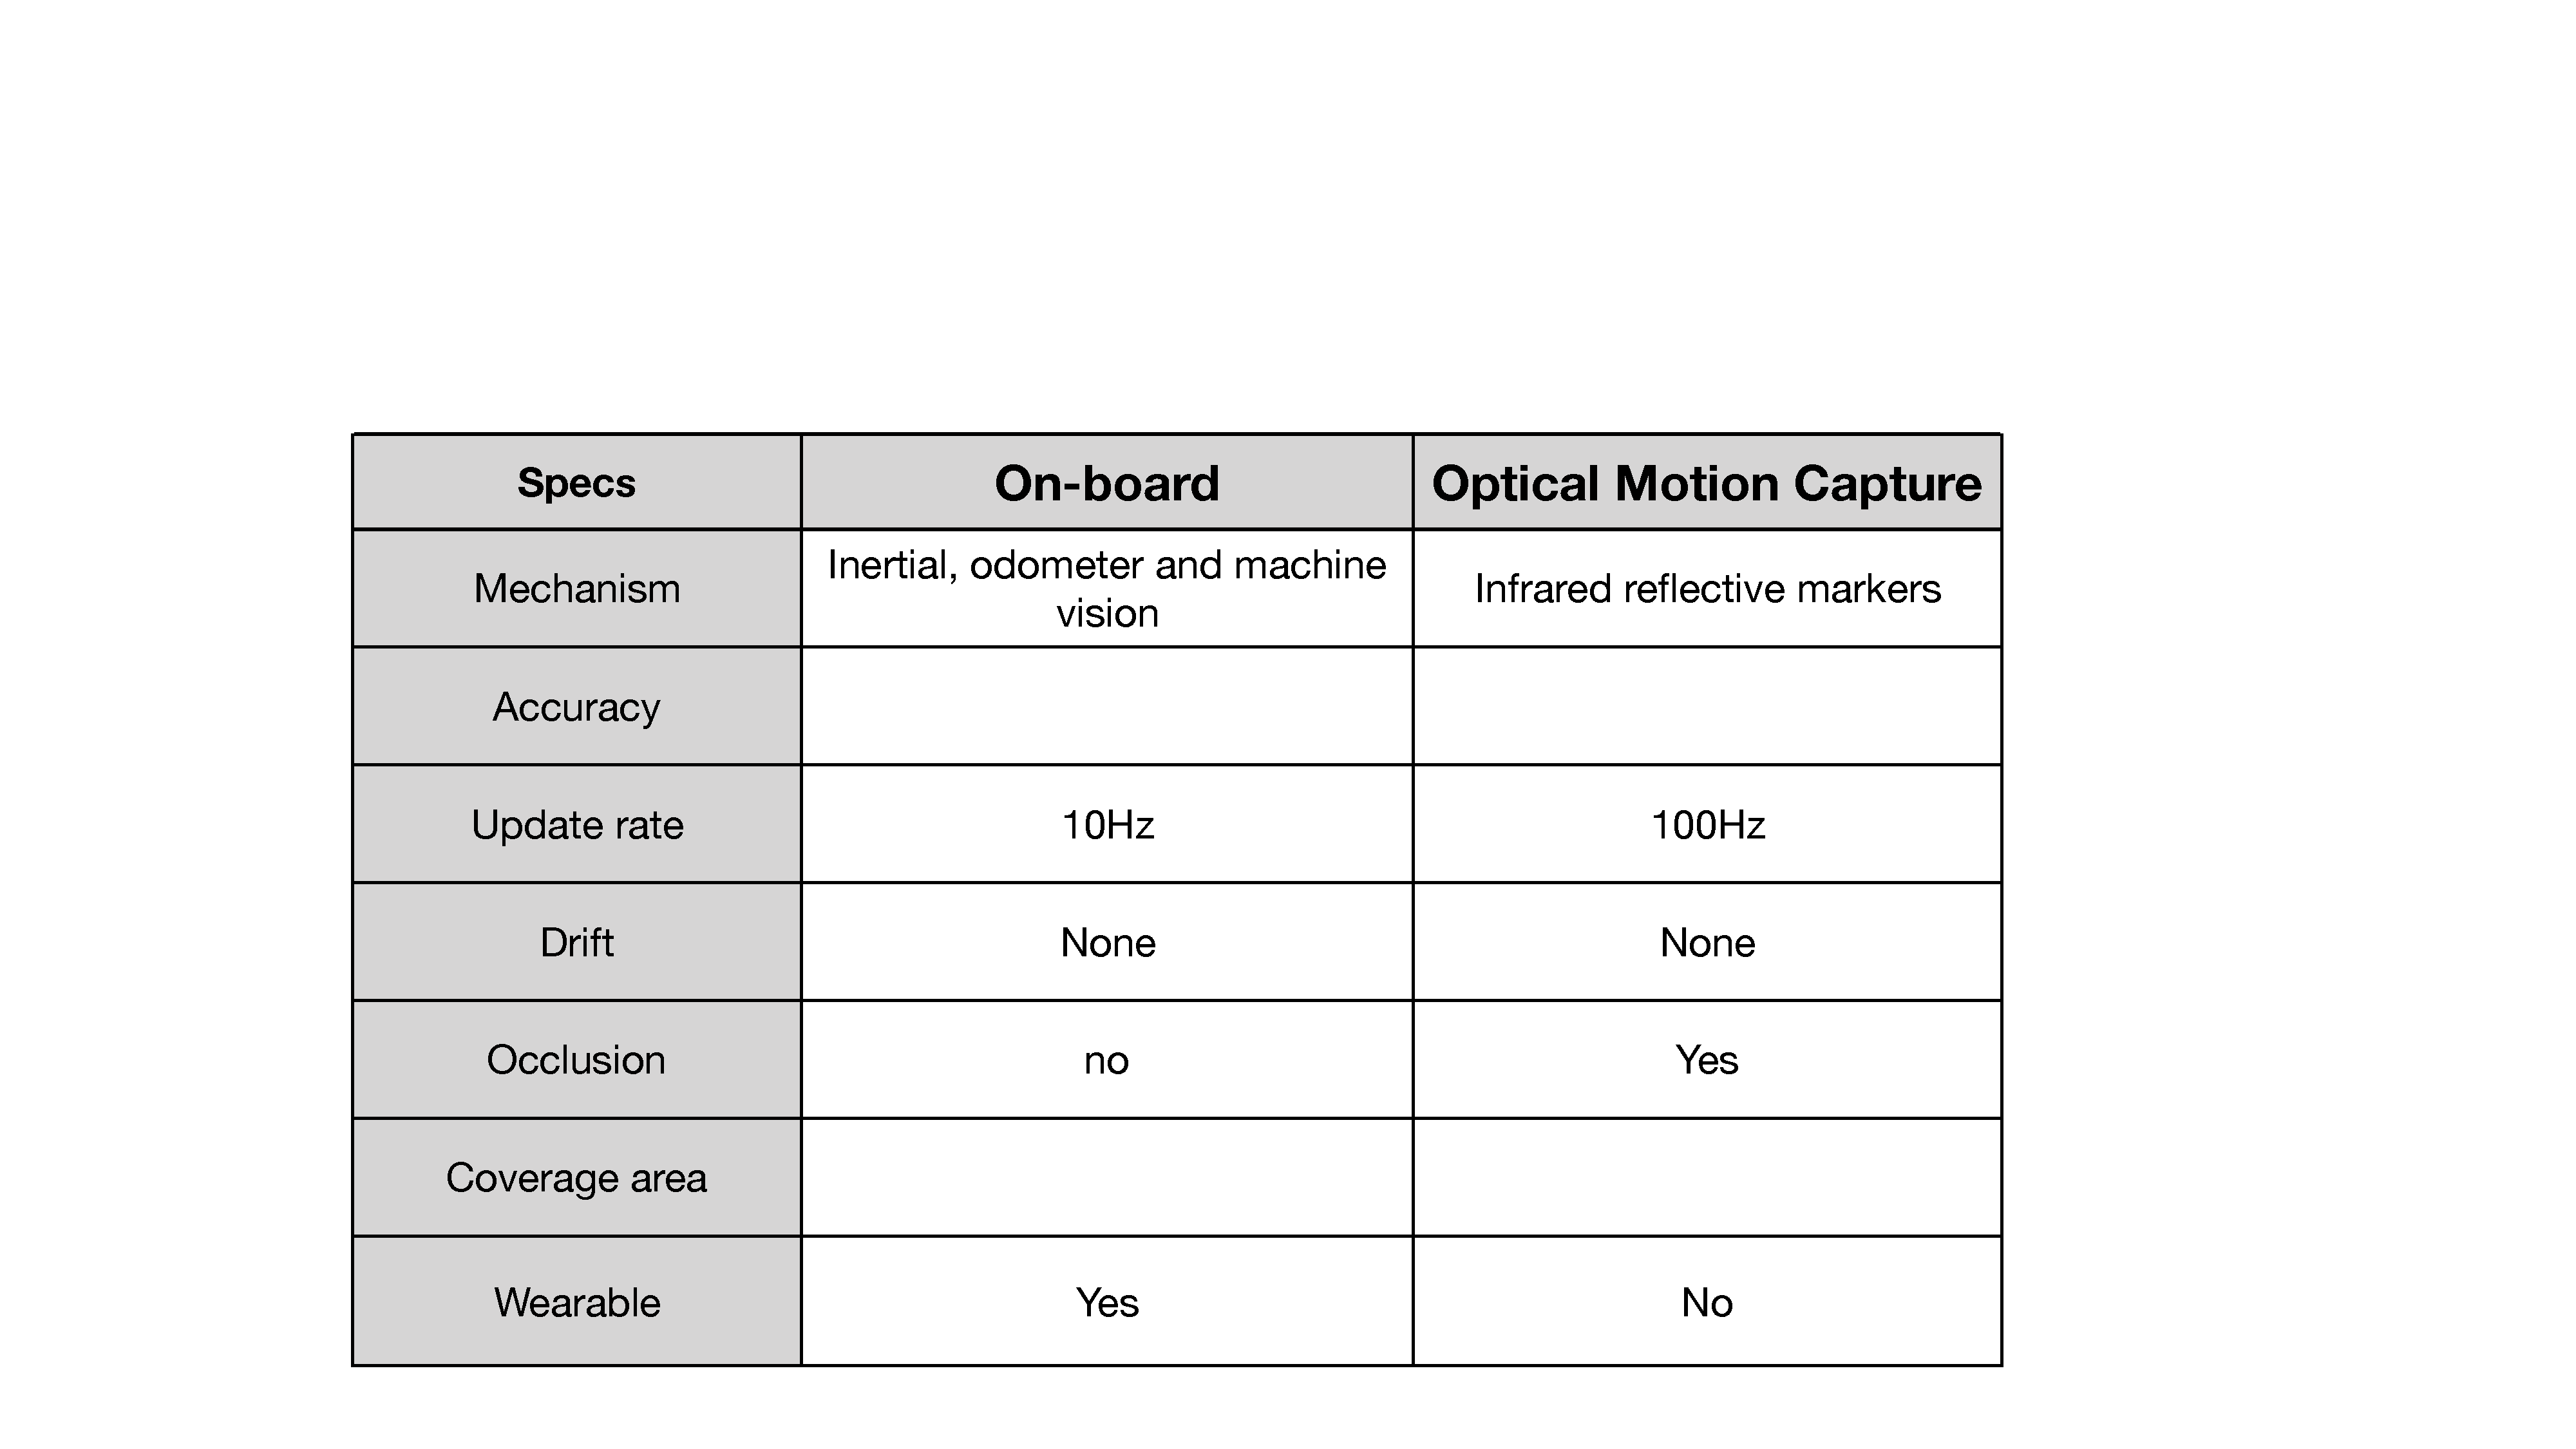
\includegraphics[width=13.0cm]{pictures/chapter5/tracking_methods_comparison.pdf}
\caption{In some cases an optical motion capture system can be used. The table provides comaprison between the on-board navigation systems and using external optical motion capture system.}
\label{fig:localization_comparison}
\end{figure}



\begin{figure}[!ht]
\centering
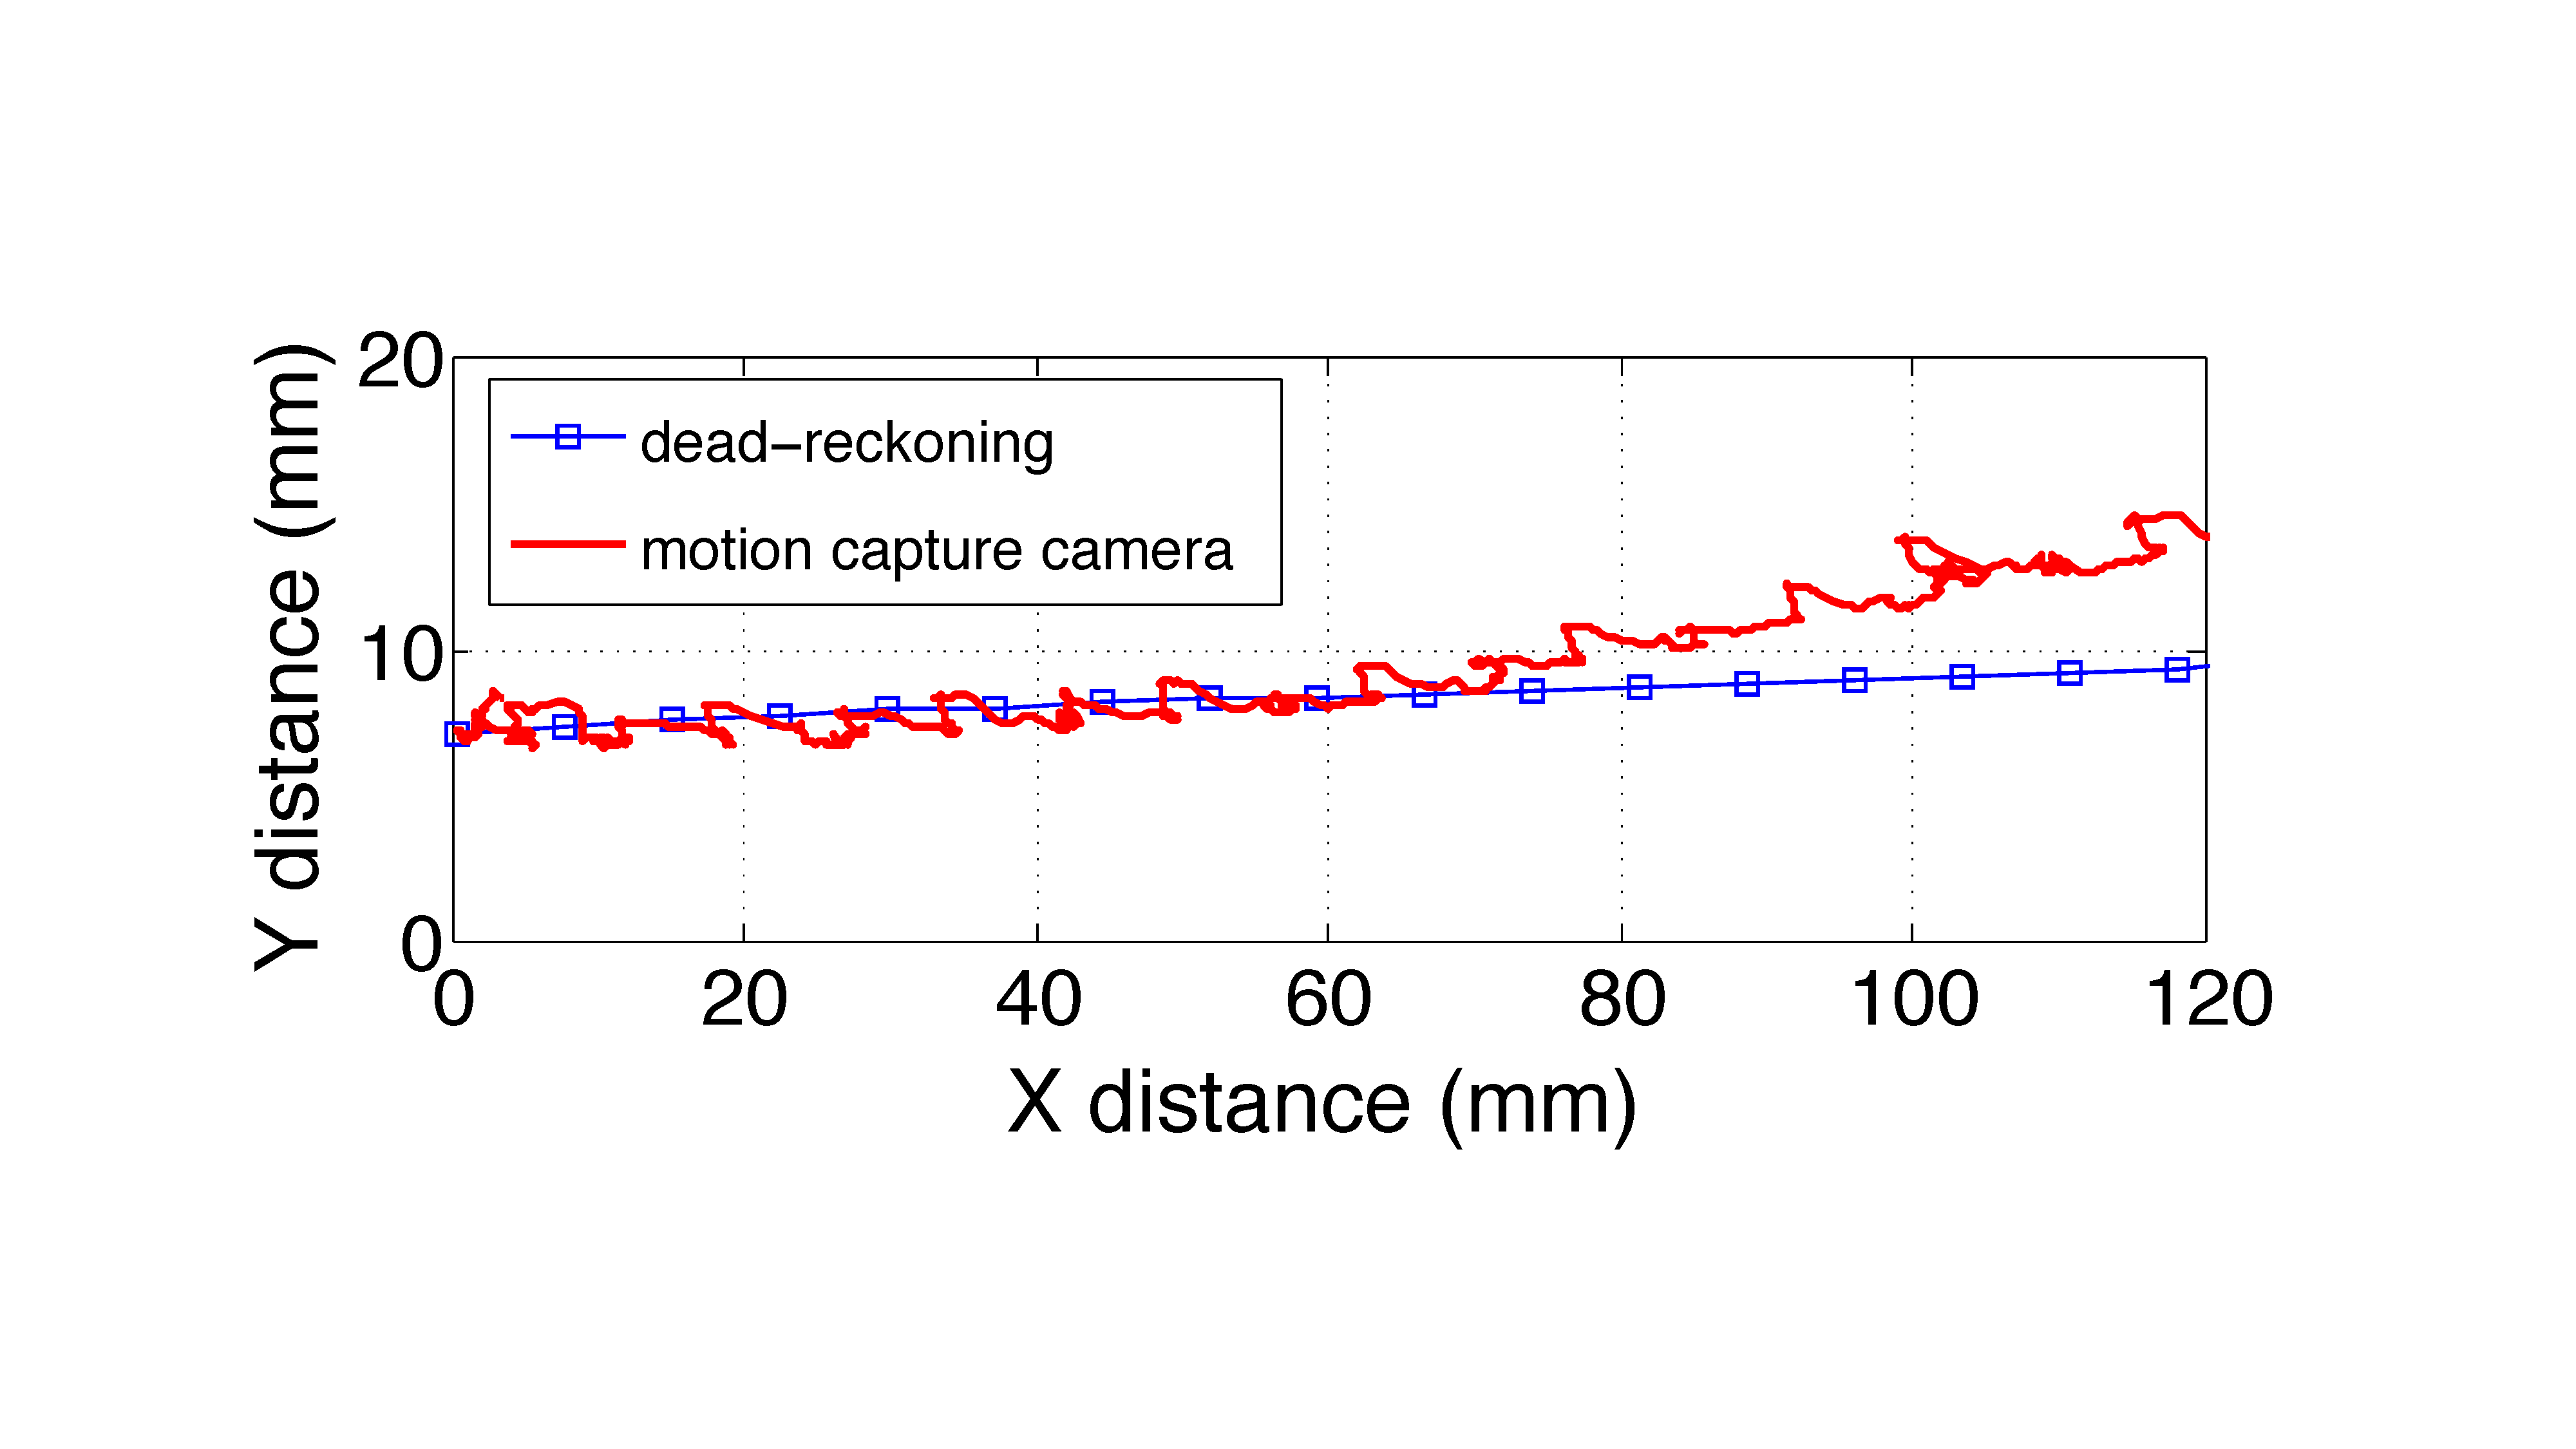
\includegraphics[width=13.0cm]{pictures/chapter5/skin_bot_localization_error.pdf}
\caption{Example of SkinBot localization with the dead-reckoning approach (blue) and a motion capture system (red).}
\label{fig:localization_skin_bot_error}
\end{figure}

\begin{figure}[!ht]
\centering
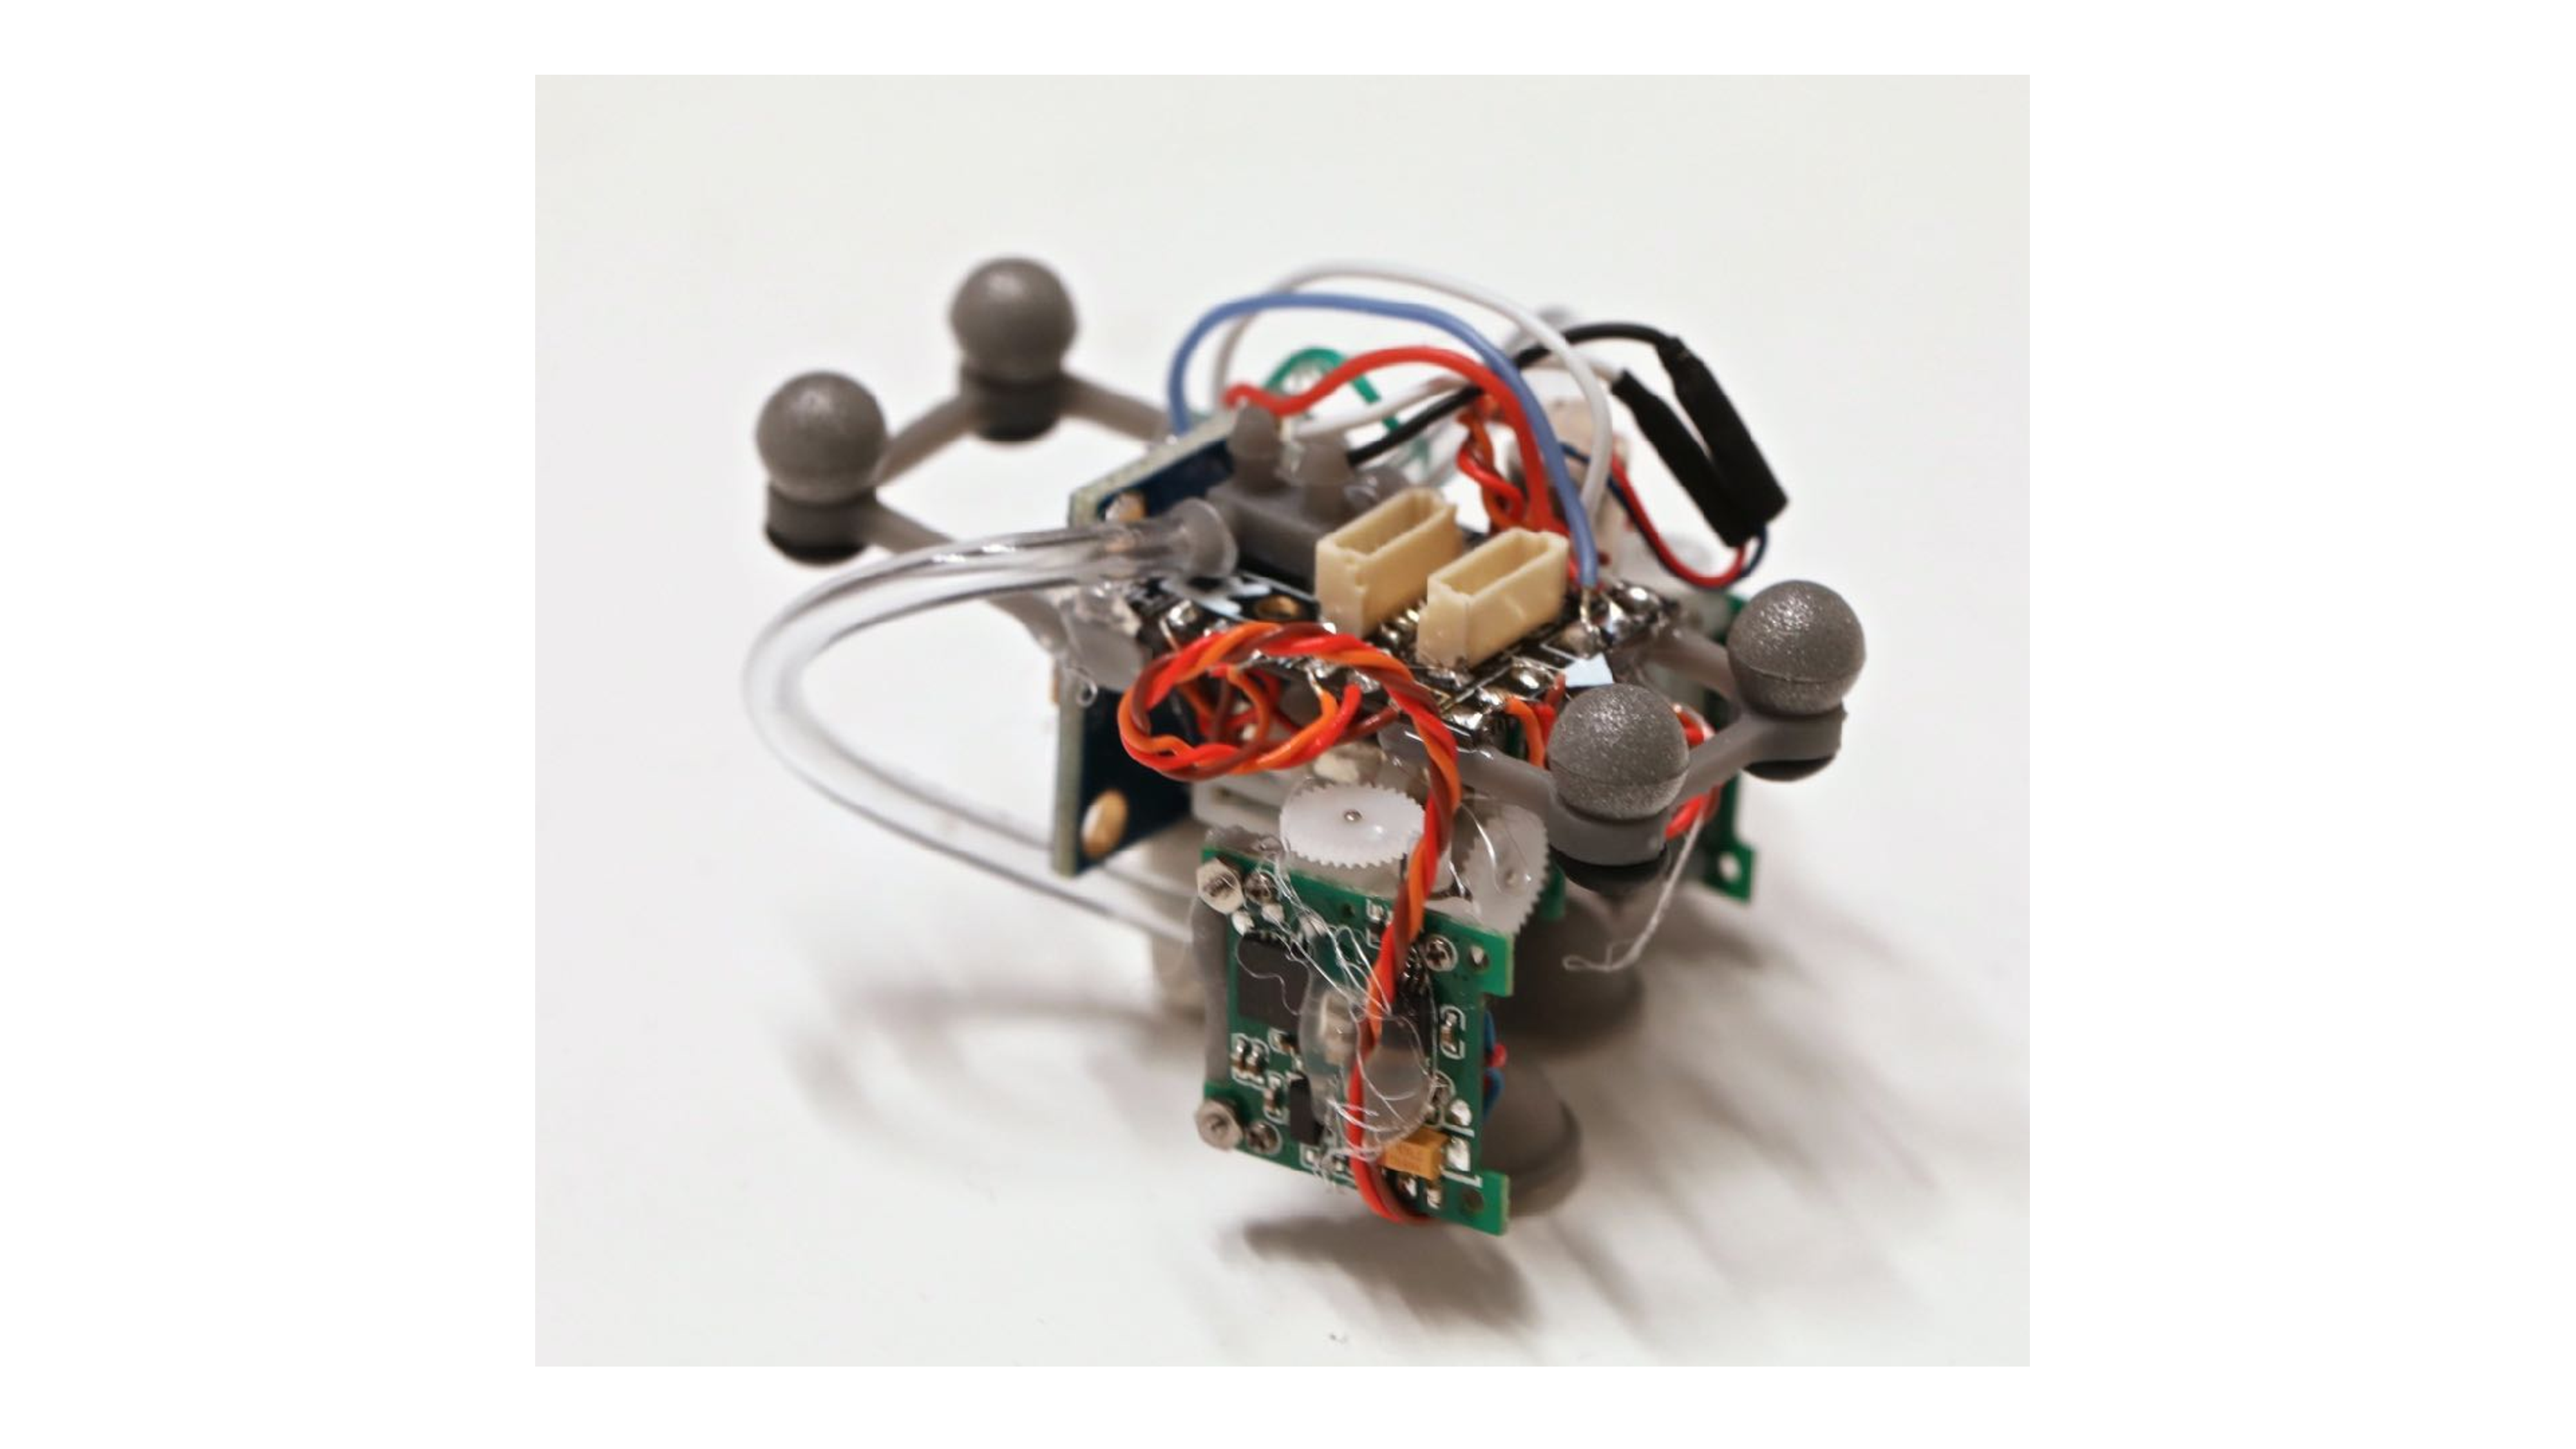
\includegraphics[width=9.0cm]{pictures/chapter5/skinbot_reflective_markers.pdf}
\caption{SkinBot with four reflective markers for optical tracking}
\label{fig:skinbot_reflective_markers}
\end{figure}




\section{Evaluation}
In this section, we describe how the localization systems were evaluated.
\subsection{Cloth robot}
As shown in Figure~\ref{fig:localization_accuracy_rovables}, we tested localization accuracy using onboard sensors and a reference camera. The path was recorded on a calibration fabric, which is shown in Figure~\ref{fig:test_bed}. The robot's movement from the camera was manually analyzed and was assumed to be the ground truth. We found that our localization algorithm has a mean error of 19.5mm and a standard deviation of 10.3mm. As Figure~\ref{fig:localization_accuracy_rovables} shows, there is an error is both linear distance (encoders) and yaw angle (IMU).

The possible sources of error include limited resolution of the encoder (2.4mm) and wheel slippage. Furthermore, the IMU had a yaw angle error of about 6.4 degrees, as measured with reference angles as the ground truth. The IMU did not experience drift, as on-chip algorithms corrected for it. 

After testing the robot on a 2D sheet, we developed a 3D testbed, as shown in~\ref{fig:3d_rovables_navigation}. This setup better reflected real-world usage. 

\begin{figure}[h]
\centering
  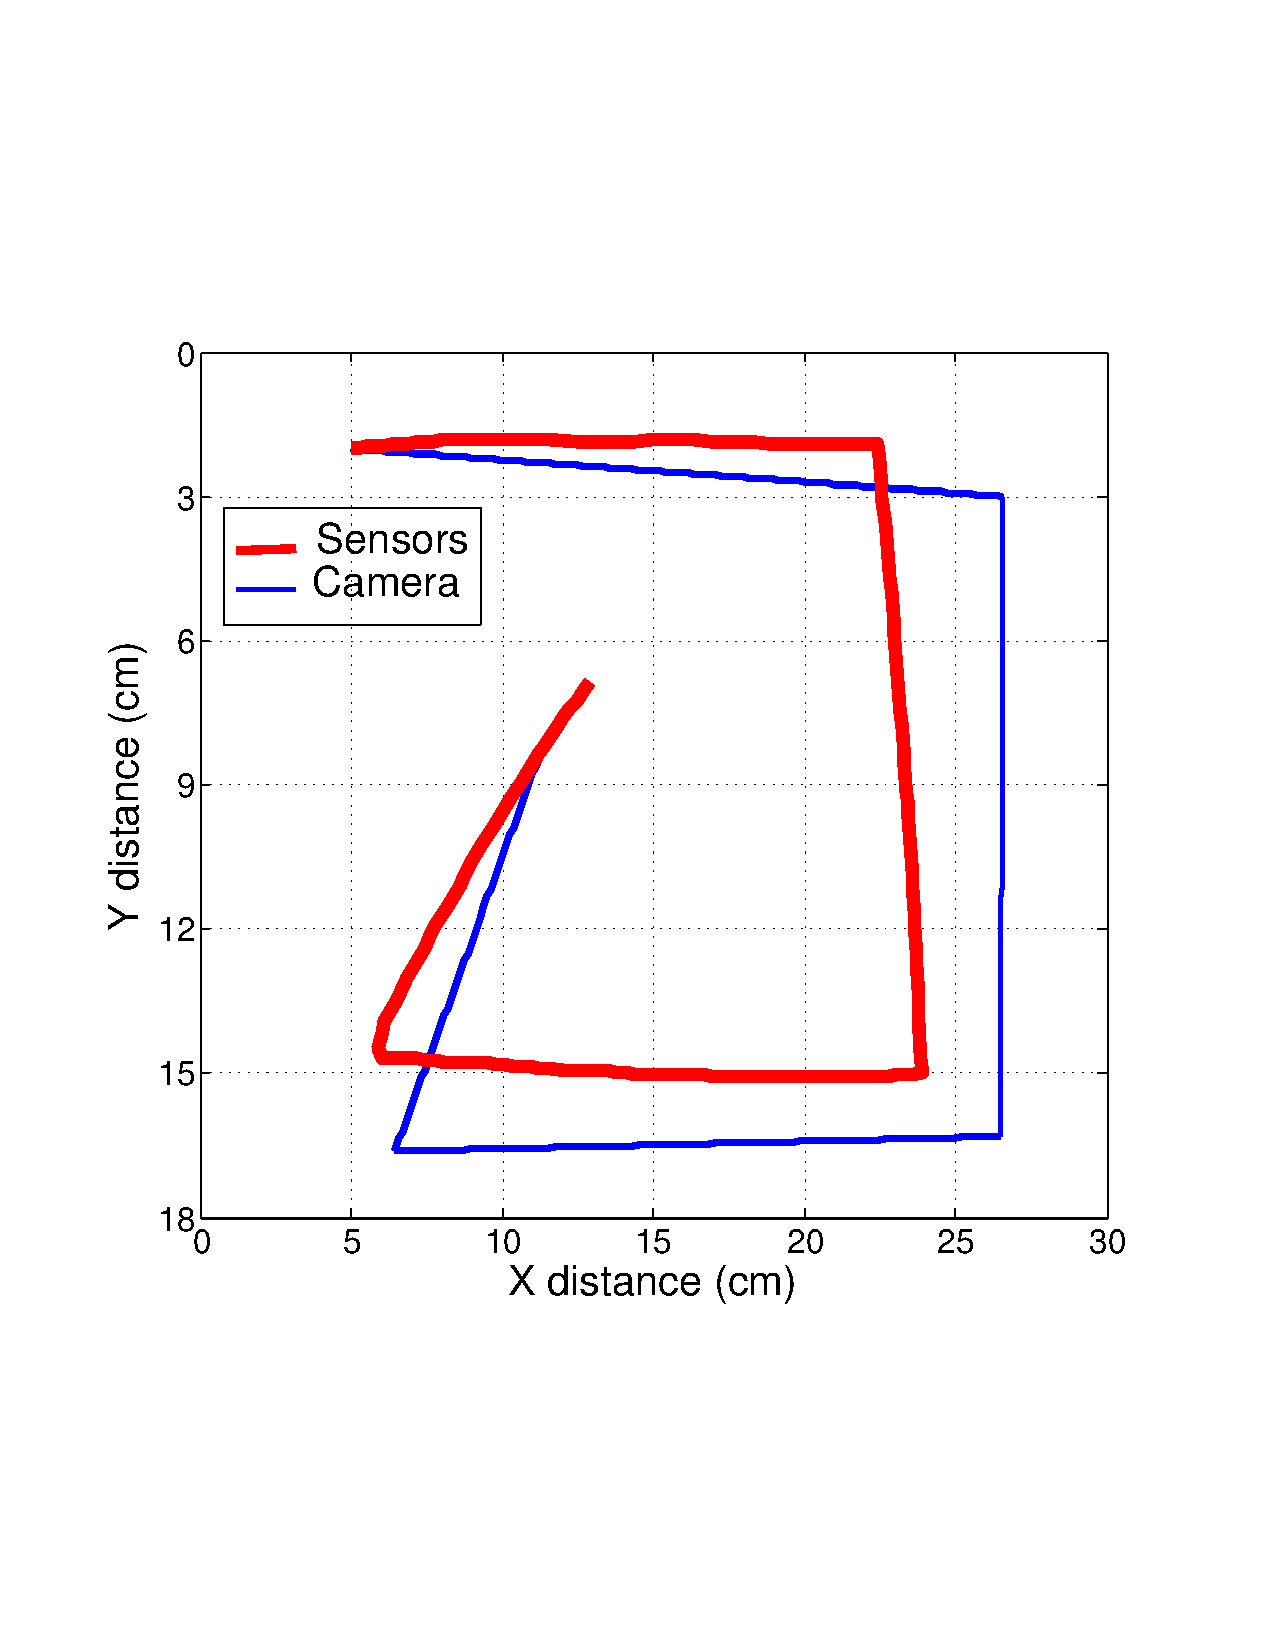
\includegraphics[width=0.7\columnwidth]{pictures/chapter5/robot_localization_v1_plot.pdf}
  \caption{Localization accuracy on a 2D fabric. Comparison of a camera (ground truth) and on-board sensors for localization of one path. }
  \label{fig:localization_accuracy_rovables}
\end{figure}

\begin{figure}[h]
\centering
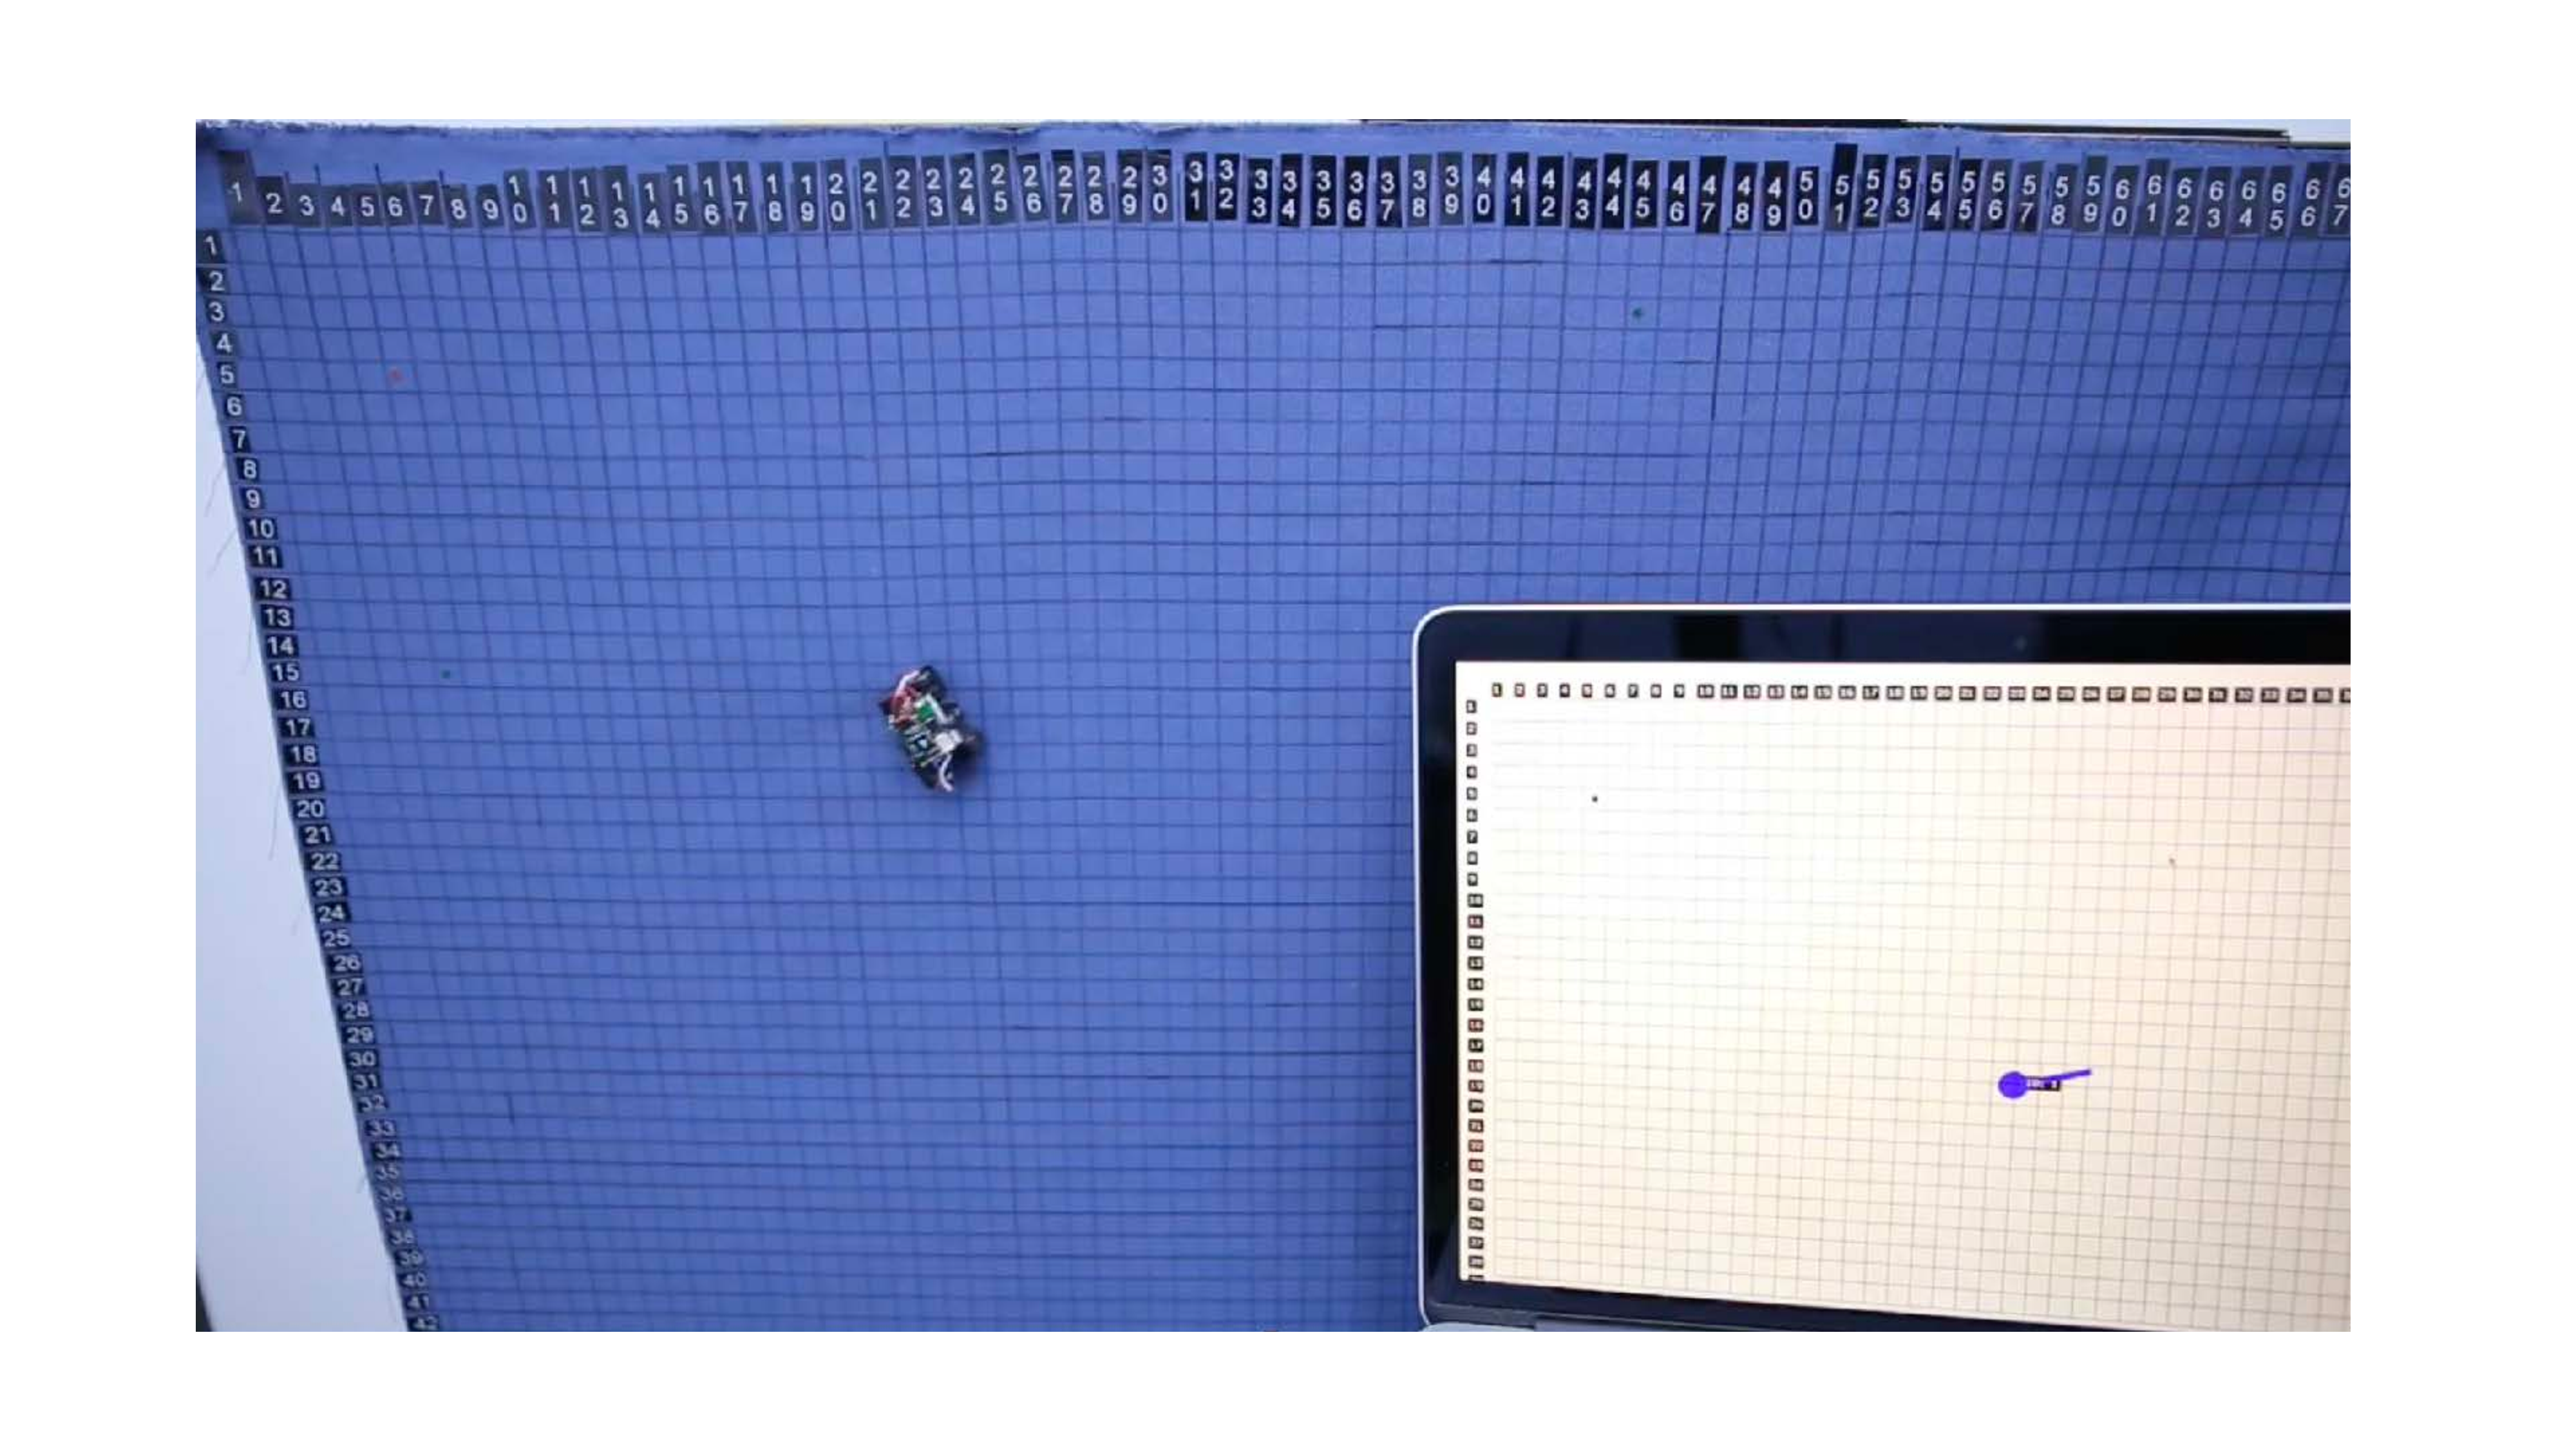
\includegraphics[width=0.9\columnwidth]{pictures/chapter5/rovable_fabric_navigation.pdf}
\caption{Fabric test bed used to develop the navigation and control algorithms }
\label{fig:test_bed}
\end{figure}

\begin{figure}[h]
\centering
  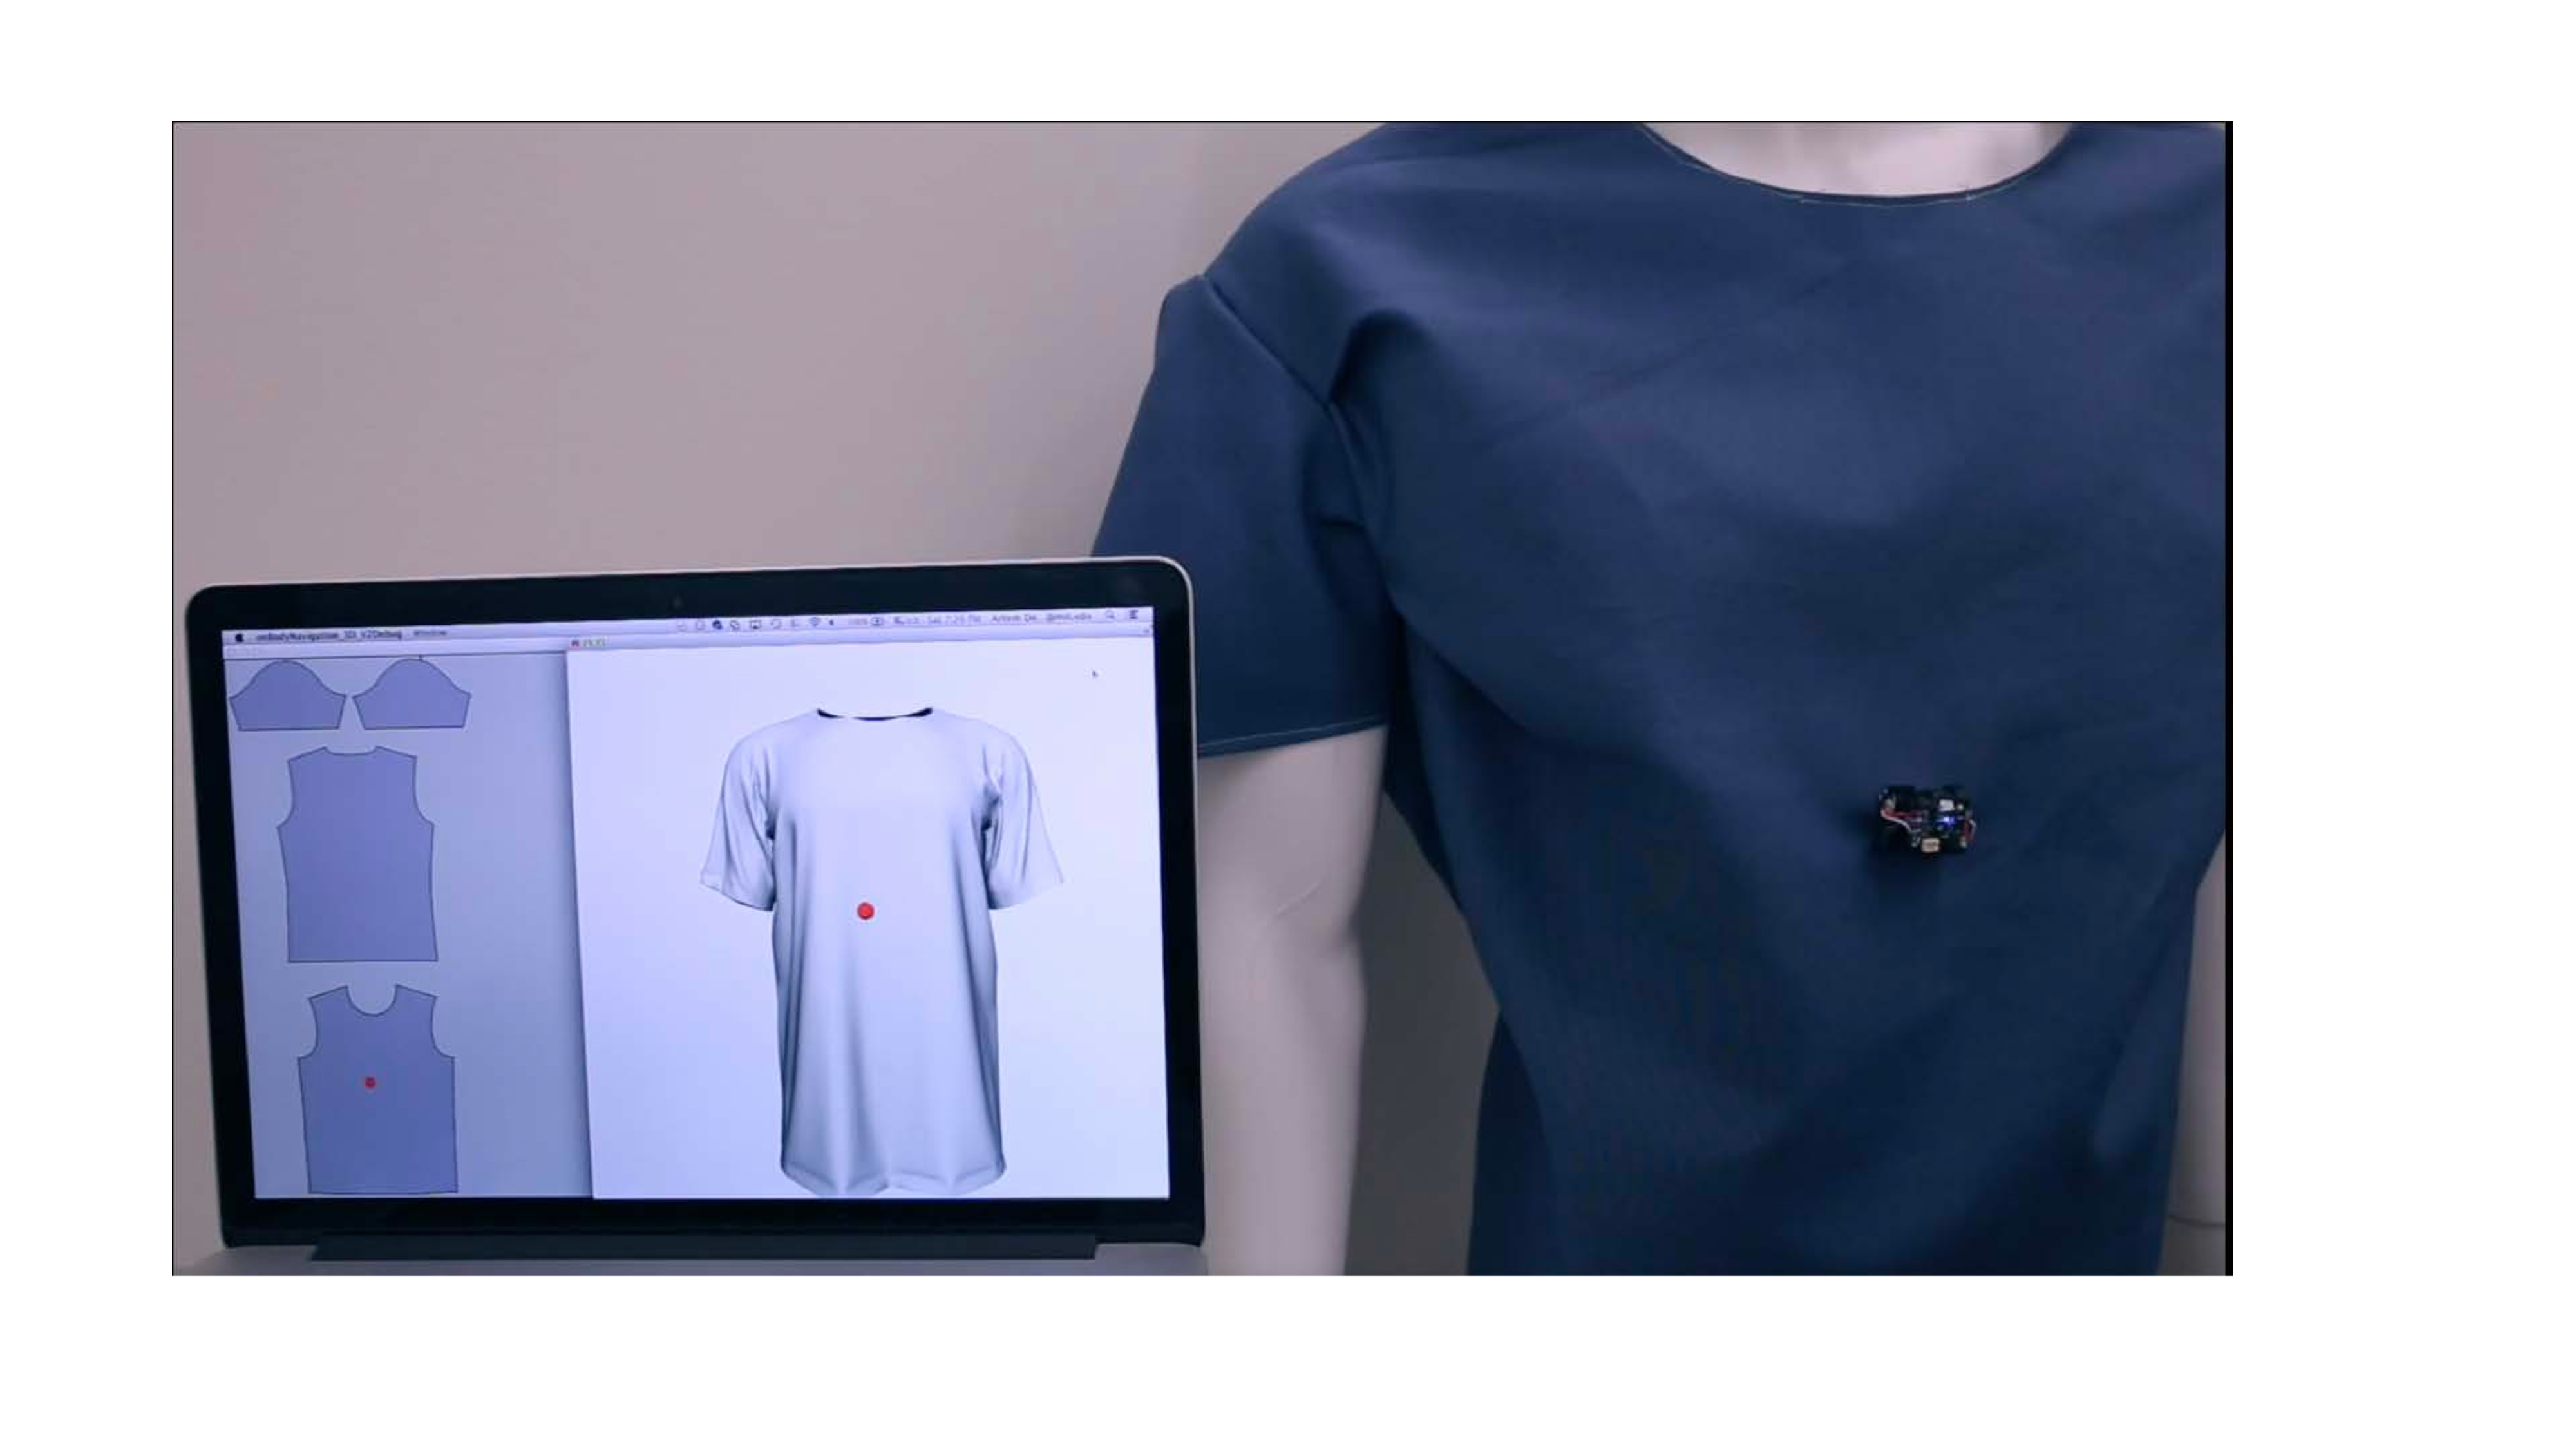
\includegraphics[width=0.9\columnwidth]{pictures/chapter5/3d_rovables_navigation.pdf}
  \caption{Localization of the robot on a fabric in 3D space. }~\label{fig:3d_rovables_navigation}
\end{figure}


\subsection{Skin robot}
To evaluate on-body robot localization, we collected data of SkinBot moving horizontally on the forearm for 20 cm and repeated the process three times. SkinBot was initially placed on a navigation marker. Gold standard localization was obtained by adding four infrared reflective markers on the robot and using a camera-based motion tracking system (Flex 13, OptiTrack). After the three repetitions, the mean error of the dead-reckoning algorithm was 4.60mm (SD:$\pm4.1$mm). Figure~\ref{fig:localization_skin_bot_error} shows an example of localization with the onboard sensors (blue) and the motion tracking system (red). One of the main sources of discrepancy between the two measures is due to the angle error from the gyroscope. In particular, the robot experienced some wobbling while moving (visible in motion tracking data), which slightly affected its heading. As expected, there was also a cumulative error as the robot moved at a rate of 0.63mm per step. To address this, SkinBot needs to recalibrate its position using the skin markers occasionally. To do so, the robot has to find at least a small piece of the marker in the camera's field of view. As the field of view is limited to about 18x18mm., the onboard localization accuracy should be under 18mm. Considering the position drift, the robot will need recalibration after 21 cm of locomotion.

%-----FABRIC------
%\section{Fabric Navigation}

%\subsection{Evaluation}
%As shown in Figure~\ref{navigation}, we made a fabric test-bed and corresponding software for testing the path planning and navigation. The test-bed was mounted vertically, to reflect actual usage. 





\section{Discussion}

%\subsection{Navigation markers}
%We have considered different navigat



\subsection{Fully autonomous operation}
In here, I will describe how the fully autonomous operation should function. 
Since mobiles phones are ubiquitous and powerful they can act as a base station for the robots. The phone provides high-level control of the robots. The phone would be loaded with the map, either from the 3D scan or garment manufacturer.  The robots would communicate to the phone through Bluetooth. 

Before activating the robots, the user would put on the markers. The phone augmented camera guide would be used to help to put the markers in the right location. Some clothing might already have the markers woven in, so no manual placement would be needed. 

Once the markers are attached, the user would place the robots on the markers. At this point the robots would go about their business using dead-reckoning, occasionally going to the markers to recalibrate. If the robots sudden user movements, they would stop and wait until there is no movement. 

\subsection{Localization accuracy}
Accurate body localization of robots proved to be more challenging than expected. We showed that body localization can be done with the onboard inertial tracking and vision markers, but it only allowed for around 21 cm of locomotion before the position drift became significant. While one marker should be sufficient to locomote on smaller areas such as the forearm, upper arm, or the upper leg, multiple markers would be required to locomote larger surfaces such as the torso. Also, inertial navigation only works on a stationary body which requires the robot to stop locomoting whenever large motion is detected.

While we hope the onboard navigation will improve in the future, whole body location is still better addressed with an external setup such as the infrared tracking system that was used in our experiments. Alternatively, epidermal robots could be teleoperated with an external camera view.    

There is a number of things that can improve the localization accuracy. Many practical localization systems use Kalman or particle filters, where multiple types of input are fused to increase accuracy. For example, to estimate the rotation of the robot encoder readings, motor commands, and IMU data can be fused to provide a better estimate. 

\subsection{Navigation without markers}
Usage of navigation markers unavoidably makes the system harder to use. It would be favorable not to use any markers. The human body contains a lot of unique features that could potentially serve as markers. Potentially, the birthmarks that were captured during the 3D scan can be used as navigation markers. Also, it might be interesting to look at blood vessels, as they can provide unique structures. Also, biosignals such as biopotentials can provide a rough location. For example, the EEG signal on the chest and near the heart is different than on the arm. 

\section{Navigation summary}
Accurate localization is essential for autonomous operation of the DWT robots. This chapter provided an overview of potential navigation methods. Unfortunately, none of the existing methods are directly applicable to the on-body scenario. Therefore, we developed a novel navigation method that utilizes both dead-reckoning with IMU and position sensors and optical markers for absolute positioning. Initial testing provided promising results ($<$10mm error), but deployment in the real-world will require greater robustness. We are hopeful that MEMS inertial sensors will significantly improve in the near future. 
